% bisect
% =====================================================================
%  EPD-SDIA-4112 -- Statistique Bayesienne -- Master 1 SDIA
%  Preambule commun aux 5 chapitres
%  Moteur : XeLaTeX (Tectonic) -- compilation : voir build.py
% =====================================================================
\documentclass[10pt,aspectratio=169]{beamer}

\usepackage{fontspec}
\usepackage{polyglossia}
\setdefaultlanguage{french}
\usepackage{amsmath,amssymb,mathtools}
\usepackage{unicode-math}
\usepackage{booktabs}
\usepackage{array}
\usepackage{colortbl}
\usepackage{xcolor}
\usepackage{tikz}
\usetikzlibrary{arrows.meta,positioning,calc,shapes.geometric,fit,backgrounds,patterns}
\usepackage{pgfplots}
\pgfplotsset{compat=1.18}
\usepgfplotslibrary{fillbetween}
\usepackage{graphicx}
\usepackage{listings}
\usepackage[most]{tcolorbox}
\tcbuselibrary{skins,breakable}
\usepackage{fontawesome5}
\usepackage{multicol}
\usepackage{multirow}
\usepackage{animate}

% ---------------------------------------------------------------- theme
\usetheme{default}
\usecolortheme{default}
\setbeamertemplate{navigation symbols}{}

\definecolor{byDeep}   {HTML}{10243E}
\definecolor{byBlue}   {HTML}{1F6FEB}
\definecolor{byCyan}   {HTML}{12A594}
\definecolor{byOrange} {HTML}{D97706}
\definecolor{byRed}    {HTML}{C0392B}
\definecolor{byGreen}  {HTML}{1E8449}
\definecolor{byPurple} {HTML}{6C5CE7}
\definecolor{byGrey}   {HTML}{5B6470}
\definecolor{byLight}  {HTML}{F4F6F8}

\setbeamercolor{frametitle}{bg=byDeep,fg=white}
\setbeamercolor{structure}{fg=byBlue}
\setbeamercolor{normal text}{fg=byDeep}
\setbeamercolor{alerted text}{fg=byRed}
\setbeamercolor{title}{fg=white}
\setbeamercolor{subtitle}{fg=white}
\setbeamercolor{author}{fg=white}
\setbeamercolor{date}{fg=white}
\setbeamercolor{item}{fg=byBlue}
\setbeamercolor{section in toc}{fg=byDeep}
\setbeamercolor{block title}{bg=byBlue!12,fg=byDeep}
\setbeamercolor{block body}{bg=byBlue!5}

\setbeamerfont{frametitle}{size=\large,series=\bfseries}
\setbeamerfont{title}{size=\LARGE,series=\bfseries}
\setbeamerfont{block title}{series=\bfseries}

% gain de place vertical : le titre de frame est suivi d'un espace negatif
% (les supports sont denses ; cela evite que le dernier encadre morde sur le pied de page)
\addtobeamertemplate{frametitle}{}{\vspace*{-4.0mm}}
\setlength{\abovedisplayskip}{3pt}
\setlength{\belowdisplayskip}{3pt}
\setlength{\abovedisplayshortskip}{2pt}
\setlength{\belowdisplayshortskip}{2pt}

\setbeamertemplate{itemize item}{\small\raise0.2ex\hbox{\textcolor{byBlue}{$\blacktriangleright$}}}
\setbeamertemplate{itemize subitem}{\tiny\raise0.35ex\hbox{\textcolor{byCyan}{$\bullet$}}}
\setlength{\tabcolsep}{3pt}   % tableaux plus etroits (les slides sont denses)
% listes plus compactes : les supports sont denses et le pied de page mange de la place
\setbeamertemplate{itemize/enumerate body begin}{\vspace*{-2.0mm}}
\setbeamertemplate{itemize/enumerate subbody begin}{\vspace*{-0.6mm}}
\setbeamertemplate{enumerate item}{\textcolor{byBlue}{\bfseries\insertenumlabel.}}
\setbeamertemplate{caption}[numbered]

% footer : chapitre | slide n/N
\setbeamertemplate{footline}{%
  % Beamer reserve la hauteur de cette boite comme zone interdite : le vskip
  % ci-dessous cale la zone de texte exactement au-dessus de la barre visible.
  \vskip 10mm%
  \leavevmode%
  \hbox{%
    \begin{beamercolorbox}[wd=.42\paperwidth,ht=1.9ex,dp=0.8ex,leftskip=.3cm]{author in head/foot}%
      \usebeamerfont{author in head/foot}\color{white}\scriptsize\insertshorttitle
    \end{beamercolorbox}%
    \begin{beamercolorbox}[wd=.42\paperwidth,ht=1.9ex,dp=0.8ex,center]{title in head/foot}%
      \usebeamerfont{title in head/foot}\color{white}\scriptsize\insertsectionhead
    \end{beamercolorbox}%
    \begin{beamercolorbox}[wd=.16\paperwidth,ht=1.9ex,dp=0.8ex,rightskip=.3cm]{date in head/foot}%
      \usebeamerfont{date in head/foot}\color{white}\scriptsize\insertframenumber\,/\,\inserttotalframenumber
    \end{beamercolorbox}}%
  \vskip0pt%
}
\setbeamercolor{author in head/foot}{bg=byDeep}
\setbeamercolor{title in head/foot}{bg=byDeep!88}
\setbeamercolor{date in head/foot}{bg=byDeep!76}

\setbeamertemplate{title page}{%
  \begin{tikzpicture}[remember picture,overlay]
    \fill[byDeep] (current page.north west) rectangle (current page.south east);
    \fill[byBlue,opacity=.30] (current page.north east) ++(-3.2,-1.1) circle (5.4cm);
    \fill[byCyan,opacity=.18] (current page.south west) ++(2.2,1.0) circle (4.2cm);
  \end{tikzpicture}
  \vspace{1.1cm}
  \begin{center}
    {\usebeamerfont{title}\usebeamercolor[fg]{title}\inserttitle\par}
    \vspace{.25cm}
    {\large\color{byCyan}\insertsubtitle\par}
    \vspace{.7cm}
    {\color{white}\small\insertauthor\par}
    \vspace{.15cm}
    {\color{white!80}\footnotesize\insertinstitute\par}
    \vspace{.15cm}
    {\color{white!70}\footnotesize\insertdate\par}
  \end{center}
}

% ------------------------------------------------------- boites maison
\newtcolorbox{qbox}[1][QUIZ]{%
  enhanced,colback=byOrange!7,colframe=byOrange,boxrule=.9pt,arc=2mm,
  left=2mm,right=2mm,top=3.4mm,bottom=1.2mm,
  title={\faQuestionCircle\ \bfseries #1},fonttitle=\bfseries\scriptsize\color{white},
  colbacktitle=byOrange,attach boxed title to top left={xshift=3mm,yshift=-2mm},
  boxed title style={arc=1mm,boxrule=0pt}}

\newtcolorbox{abox}[1][ACTIVITE]{%
  enhanced,colback=byBlue!6,colframe=byBlue,boxrule=.9pt,arc=2mm,
  left=2mm,right=2mm,top=3.4mm,bottom=1.2mm,
  title={\faUsers\ \bfseries #1},fonttitle=\bfseries\scriptsize\color{white},
  colbacktitle=byBlue,attach boxed title to top left={xshift=3mm,yshift=-2mm},
  boxed title style={arc=1mm,boxrule=0pt}}

\newtcolorbox{ebox}[1][EXEMPLE]{%
  enhanced,colback=byGreen!6,colframe=byGreen,boxrule=.9pt,arc=2mm,
  left=2mm,right=2mm,top=3.4mm,bottom=1.2mm,
  title={\faFlask\ \bfseries #1},fonttitle=\bfseries\scriptsize\color{white},
  colbacktitle=byGreen,attach boxed title to top left={xshift=3mm,yshift=-2mm},
  boxed title style={arc=1mm,boxrule=0pt}}

\newtcolorbox{kbox}[1][A RETENIR]{%
  enhanced,colback=byPurple!6,colframe=byPurple,boxrule=.9pt,arc=2mm,
  left=2mm,right=2mm,top=3.4mm,bottom=1.2mm,
  title={\faLightbulb\ \bfseries #1},fonttitle=\bfseries\scriptsize\color{white},
  colbacktitle=byPurple,attach boxed title to top left={xshift=3mm,yshift=-2mm},
  boxed title style={arc=1mm,boxrule=0pt}}

\newtcolorbox{wbox}[1][ATTENTION]{%
  enhanced,colback=byRed!6,colframe=byRed,boxrule=.9pt,arc=2mm,
  left=2mm,right=2mm,top=3.4mm,bottom=1.2mm,
  title={\faExclamationTriangle\ \bfseries #1},fonttitle=\bfseries\scriptsize\color{white},
  colbacktitle=byRed,attach boxed title to top left={xshift=3mm,yshift=-2mm},
  boxed title style={arc=1mm,boxrule=0pt}}

\newtcolorbox{solbox}[1][SOLUTION]{%
  enhanced,colback=byCyan!7,colframe=byCyan,boxrule=.9pt,arc=2mm,
  left=2mm,right=2mm,top=3.4mm,bottom=1.2mm,
  title={\faCheckCircle\ \bfseries #1},fonttitle=\bfseries\scriptsize\color{white},
  colbacktitle=byCyan,attach boxed title to top left={xshift=3mm,yshift=-2mm},
  boxed title style={arc=1mm,boxrule=0pt}}

\newtcolorbox{codebox}[1][Code Python]{%
  enhanced,colback=byLight,colframe=byGrey!60,boxrule=.6pt,arc=1.5mm,
  left=1.5mm,right=1.5mm,top=3.8mm,bottom=1.0mm,
  title={\faPython\ \ttfamily\small #1},fonttitle=\small\color{white},
  colbacktitle=byGrey,attach boxed title to top left={xshift=3mm,yshift=-2mm},
  boxed title style={arc=1mm,boxrule=0pt}}

\newtcolorbox{figbox}[1][]{%
  enhanced,colback=white,colframe=byDeep!25,boxrule=.6pt,arc=1.5mm,
  left=1mm,right=1mm,top=1mm,bottom=1mm,#1}

% --------------------------------------------------------- listings
\definecolor{codekw}{HTML}{0B5394}
\definecolor{codestr}{HTML}{B8531A}
\definecolor{codecom}{HTML}{57744E}
\definecolor{codebg}{HTML}{F6F8FA}
\lstdefinestyle{py}{
  language=Python,
  backgroundcolor=\color{codebg},
  basicstyle=\ttfamily\fontsize{6.6}{7.6}\selectfont,
  keywordstyle=\color{codekw}\bfseries,
  commentstyle=\color{codecom}\itshape,
  stringstyle=\color{codestr},
  numberstyle=\tiny\color{byGrey},
  numbers=left,numbersep=4pt,
  frame=none,
  breaklines=true,breakatwhitespace=false,
  showstringspaces=false,
  columns=fullflexible,keepspaces=true,
  upquote=true,
  literate={é}{{\'e}}1 {è}{{\`e}}1 {ê}{{\^e}}1 {à}{{\`a}}1 {â}{{\^a}}1
           {î}{{\^i}}1 {ô}{{\^o}}1 {û}{{\^u}}1 {ç}{{\c c}}1 {ù}{{\`u}}1
           {É}{{\'E}}1 {È}{{\`E}}1 {À}{{\`A}}1 {Ê}{{\^E}}1 {Ç}{{\c C}}1
           {œ}{{\oe}}1 {’}{{'}}1 {«}{{\guillemotleft}}1 {»}{{\guillemotright}}1
           {→}{{$\rightarrow$}}1 {α}{{$\alpha$}}1 {β}{{$\beta$}}1 {θ}{{$\theta$}}1
           {μ}{{$\mu$}}1 {σ}{{$\sigma$}}1 {λ}{{$\lambda$}}1 {π}{{$\pi$}}1
           {τ}{{$\tau$}}1 {ρ}{{$\rho$}}1 {≈}{{$\approx$}}1 {≤}{{$\leq$}}1
           {≥}{{$\geq$}}1 {×}{{$\times$}}1 {≠}{{$\neq$}}1 {∈}{{$\in$}}1
}
\lstset{style=py}

\newcommand{\py}[1]{\lstinline[style=py,basicstyle=\ttfamily\small]|#1|}
\newcommand{\file}[1]{\texttt{\small #1}}
\newcommand{\R}{\mathbb{R}}
\newcommand{\N}{\mathcal{N}}
\newcommand{\E}{\mathbb{E}}
\newcommand{\Var}{\mathrm{Var}}
\newcommand{\post}{\text{post}}
\newcommand{\like}{\text{vrais.}}
\newcommand{\data}{\mathcal{D}}
\newcommand{\given}{\,\vert\,}
\DeclareMathOperator*{\argmax}{arg\,max}
\DeclareMathOperator*{\argmin}{arg\,min}

% icones de validation
\newcommand{\ok}{\textcolor{byGreen}{\faCheckCircle}}
\newcommand{\nok}{\textcolor{byRed}{\faTimesCircle}}
\newcommand{\warn}{\textcolor{byOrange}{\faExclamationTriangle}}

% chemin des figures
\graphicspath{{../figures/}{./figures/}{figures/}{../assets/}{./assets/}}

% ------------------------------------------------ page de garde de chapitre
% A utiliser en tete de chaque fichier de chapitre : identique en build
% autonome et en build maitre (aucune dependance a \title).
\newcommand{\chapterslide}[4]{%
\begin{frame}[plain]
\begin{tikzpicture}[remember picture,overlay]
  \fill[byDeep] (current page.north west) rectangle (current page.south east);
  \fill[byBlue,opacity=.30] (current page.north east) ++(-3.0,-0.9) circle (5.0cm);
  \fill[byCyan,opacity=.16] (current page.south west) ++(2.4,1.2) circle (4.4cm);
\end{tikzpicture}
\vspace{0.55cm}
\begin{columns}[c]
% ---- logo officiel de l'ecole, dans un cartouche blanc
\begin{column}{0.20\textwidth}
  \centering
  \begin{tcolorbox}[colback=white,colframe=white,boxrule=0pt,arc=1.5mm,
     left=1mm,right=1mm,top=1mm,bottom=1mm,width=2.5cm]
    \centering
    
\includegraphics[width=2.1cm]{logo_enspd.png}
  \end{tcolorbox}
\end{column}
% ---- identification du chapitre et de l'enseignante
\begin{column}{0.76\textwidth}
  {\color{byCyan}\bfseries\large #1\par}
  \vspace{.20cm}
  {\color{white}\bfseries\Large #2\par}
  \vspace{.30cm}
  {\color{white!85}\small Statistique Bayésienne --- EPD-SDIA-4112 --- Master 1 SDIA\par}
  \vspace{.06cm}
  {\color{white!70}\footnotesize #3\par}
  \vspace{.26cm}
  {\color{byCyan}\bfseries\normalsize Enseignante : Dr. Noulapeu Ngaffo Armielle\par}
  \vspace{.06cm}
  {\color{white!80}\footnotesize École Nationale Supérieure Polytechnique de Douala\par}
  {\color{white!65}\footnotesize Université de Douala --- Département Génie Informatique
   et Télécommunications\par}
\end{column}
\end{columns}
\vspace{.30cm}
\begin{columns}[t]
\begin{column}{0.06\textwidth}\end{column}
\begin{column}{0.88\textwidth}
\begin{tcolorbox}[enhanced,colback=byDeep!62!black,colframe=byCyan!75,arc=2mm,
   boxrule=.6pt,left=2mm,right=2mm,top=1.4mm,bottom=1.4mm,coltext=white]
\small #4
\end{tcolorbox}
\end{column}
\begin{column}{0.06\textwidth}\end{column}
\end{columns}
\end{frame}}

% compteur de slides atteignables : \nb{50}
\newcommand{\nb}[1]{}


\title[Ch 1]{Introduction}
\subtitle{EPD-SDIA-4112}
\author{Test}
\institute{DGI}
\date{2026}
\begin{document}
% =====================================================================
%  EPD-SDIA-4112 -- Statistique Bayesienne -- Master 1 SDIA
%  CHAPITRE 1 : Introduction et fondements bayesiens   (50 slides, 8 h)
%  Fichier de frames : aucune dependance a \title (build maitre + build seul)
% =====================================================================
\section{Chapitre 1 --- Fondements bayésiens}

% ---------------------------------------------------------------- 1
\chapterslide{Chapitre 1}{Introduction et fondements bayésiens}{8 h --- 5 sections --- 50 slides}{%
\textbf{Objectifs} --- distinguer les deux interprétations de la probabilité ;
énoncer et appliquer le théorème de Bayes ; définir prior, vraisemblance,
posterior et loi prédictive ; écrire un premier modèle en PyMC ;
lire un intervalle de crédibilité à 95~\%.}


% ---------------------------------------------------------------- 2
\begin{frame}{Pourquoi le bayésien ?}
\begin{columns}[t]
\begin{column}{0.52\textwidth}
\begin{ebox}[Trois raisons décisives]
\begin{itemize}
  \item \textbf{Données rares} : en santé, finance ou industrie, on ne dispose
        pas de 10\,000 observations. Le prior compense.
  \item \textbf{Connaissance experte} : l'expert sait déjà quelque chose ;
        le bayésien lui donne un langage pour l'écrire.
  \item \textbf{Incertitude honnête} : on répond par
        « $P(\theta > 0{,}5 \given y) = 0{,}97$ », pas par un rejet binaire.
\end{itemize}
\end{ebox}
\end{column}
\begin{column}{0.44\textwidth}
\begin{kbox}[Applications en M1 SDIA]
\begin{itemize}
  \item Dépistage et essais cliniques
  \item A/B testing en ligne
  \item Filtrage de spam, détection de fraude
  \item Systèmes de recommandation
  \item Modèles hiérarchiques et petits effectifs
  \item Apprentissage bayésien profond (BNN)
\end{itemize}
\end{kbox}
\end{column}
\end{columns}
\vspace{1mm}
\centering
\begin{tcolorbox}[colback=byCyan!8,colframe=byCyan,width=.94\textwidth,arc=2mm]
\centering\small
\textbf{Fil rouge du cours :} transformer une croyance a priori en
\textbf{distribution de probabilité} sur le paramètre, puis la mettre à jour par les données.
\end{tcolorbox}
\end{frame}

% ---------------------------------------------------------------- 3
\begin{frame}{Le problème qui met tout le monde d'accord}
\begin{columns}[t]
\begin{column}{0.48\textwidth}
\begin{ebox}[Énoncé]
Un test de dépistage a
\begin{itemize}
  \item sensibilité $P(T^+ \given M) = 0{,}99$
  \item spécificité $P(T^- \given \bar M) = 0{,}95$
  \item maladie rare : prévalence $P(M) = 0{,}01$
\end{itemize}
\vspace{1mm}
\textbf{Question :} le test est positif. Quelle est la probabilité d'être malade ?
\vspace{1mm}

\centering\large\textbf{Réponse intuitive la plus fréquente : 95 \%}
\end{ebox}
\end{column}
\begin{column}{0.48\textwidth}
\begin{center}
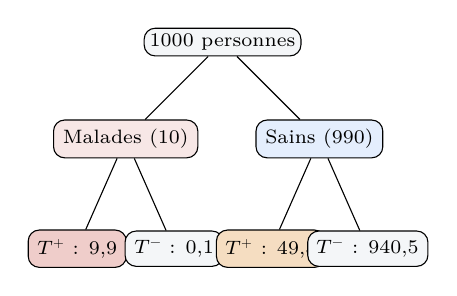
\begin{tikzpicture}[scale=.82,every node/.style={font=\scriptsize},
   level 1/.style={sibling distance=30mm,level distance=15mm},
   level 2/.style={sibling distance=15mm,level distance=17mm}]
\node[draw,rounded corners,fill=byLight,inner sep=2pt] {1000 personnes}
  child {node[draw,rounded corners,fill=byRed!12] {Malades (10)}
    child {node[fill=byRed!25,draw,rounded corners] {$T^+$ : 9,9}}
    child {node[fill=byLight,draw,rounded corners] {$T^-$ : 0,1}}}
  child {node[draw,rounded corners,fill=byBlue!12] {Sains (990)}
    child {node[fill=byOrange!25,draw,rounded corners] {$T^+$ : 49,5}}
    child {node[fill=byLight,draw,rounded corners] {$T^-$ : 940,5}}};
\end{tikzpicture}
\end{center}
\vspace{-1mm}
\begin{solbox}[Le calcul qui fâche]
\centering
$P(M \given T^+) = \dfrac{9{,}9}{9{,}9 + 49{,}5} = \mathbf{16{,}7\ \%}$
\end{solbox}
\end{column}
\end{columns}
\end{frame}

% ---------------------------------------------------------------- 4
\begin{frame}{Quiz d'ouverture (Kahoot / Mentimeter, 3 min)}
\begin{qbox}[Question 1 -- Diagnostic médical]
Même test (sensibilité 99 \%, spécificité 95 \%). La prévalence passe de 1 \% à 20 \%.
Quelle est la nouvelle probabilité d'être malade après un test positif ?
\vspace{2mm}
\begin{enumerate}
  \item[(A)] environ 17 \% \quad \textit{(inchangé : le test est le même)}
  \item[(B)] environ 83 \% \quad \checkmark
  \item[(C)] environ 99 \%
  \item[(D)] impossible à dire sans plus de données
\end{enumerate}
\vspace{2mm}
\textcolor{byBlue}{\textbf{Votez avant de calculer.}} Puis :
$P(M \given T^+) = \frac{0{,}99 \times 0{,}20}{0{,}99 \times 0{,}20 + 0{,}05 \times 0{,}80} = 0{,}832$.
\end{qbox}
\vspace{1mm}
\begin{kbox}[Le message de la séance]
La réponse ne dépend pas seulement du test : elle dépend de ce qu'on
\textbf{croyait avant}. C'est toute la statistique bayésienne en une phrase.
\end{kbox}
\end{frame}

% ---------------------------------------------------------------- 5
\begin{frame}{Trois siècles d'une idée contrariée}
\begin{center}
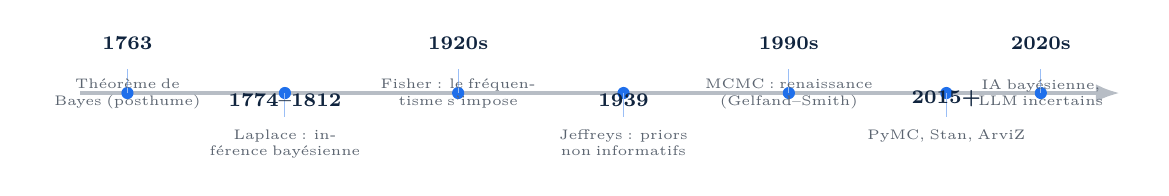
\begin{tikzpicture}[xscale=1.0,yscale=1.0]
\draw[very thick,byDeep!30,-{Latex[length=3mm]}] (0,0) -- (13.2,0);
\foreach \x/\y/\n/\t in {
   0.6/1/{1763}/{Théorème de Bayes (posthume)},
   2.6/-1/{1774--1812}/{Laplace : inférence bayésienne},
   4.8/1/{1920s}/{Fisher : le fréquentisme s'impose},
   6.9/-1/{1939}/{Jeffreys : priors non informatifs},
   9.0/1/{1990s}/{MCMC : renaissance (Gelfand--Smith)},
   11.0/-1/{2015+}/{PyMC, Stan, ArviZ},
   12.2/1/{2020s}/{IA bayésienne, LLM incertains}}
{
  \fill[byBlue] (\x,0) circle (2.2pt);
  \draw[byBlue!45] (\x,0) -- (\x,0.30*\y+0.0);
  \node[anchor=south,align=center,font=\scriptsize\bfseries,text=byDeep]
       at (\x,0.36*\y+0.06) {\n};
  \node[anchor=north,align=center,font=\tiny,text=byGrey,text width=2.3cm]
       at (\x,0.32*\y-0.02) {\t};
}
\end{tikzpicture}
\end{center}
\vspace{2mm}
\begin{ebox}[Pourquoi si longtemps ?]
\begin{itemize}
  \item Le calcul bayésien exige des intégrales $\int p(\theta) p(y \given \theta)\,\mathrm{d}\theta$,
        souvent sans forme close.
  \item Les ordinateurs et les algorithmes MCMC (chapitre 5) ont levé ce verrou
        \textbf{à la fin des années 1980}.
  \item Aujourd'hui une régression bayésienne tient en cinq lignes de \py{pm.sample()}.
\end{itemize}
\end{ebox}
\end{frame}
% ---------------------------------------------------------------- 6
\begin{frame}{Objectifs pédagogiques du chapitre}
\begin{columns}[t]
\begin{column}{0.48\textwidth}
\begin{kbox}[Savoirs]
\begin{itemize}
  \item Distinguer les deux interprétations de la probabilité
  \item Énoncer et démontrer le théorème de Bayes
  \item Définir prior, vraisemblance, posterior, prédictive
  \item Lire un intervalle de crédibilité
\end{itemize}
\end{kbox}
\end{column}
\begin{column}{0.48\textwidth}
\begin{abox}[Savoir-faire évalués]
\begin{itemize}
  \item Calculer un posterior conjugué à la main
  \item \textbf{Écrire et exécuter} un modèle PyMC
  \item Produire un graphique de posterior exploitable
  \item Critiquer un prior (trop informatif ? justifié ?)
\end{itemize}
\end{abox}
\end{column}
\end{columns}
\vspace{2mm}
\begin{tcolorbox}[colback=byLight,colframe=byGrey!50,arc=2mm,width=.95\textwidth]
\centering\small
\textbf{Évaluation} — contrôle continu 30 \% (TP noté + quiz) \;|\; examen final écrit 70 \%.
\end{tcolorbox}
\end{frame}

% ---------------------------------------------------------------- 7
\begin{frame}{Plan du chapitre 1 (8 h)}
\begin{enumerate}
  \item[1.1] \textbf{Contexte et motivation} \hfill \textit{slides 2--8}
  \item[1.2] \textbf{Probabilité : deux interprétations} \hfill \textit{slides 9--20}
  \item[1.3] \textbf{Le théorème de Bayes et sa mécanique} \hfill \textit{slides 21--34}
  \item[1.4] \textbf{Bayésien contre fréquentiste} \hfill \textit{slides 35--44}
  \item[1.5] \textbf{L'écosystème logiciel et le premier modèle} \hfill \textit{slides 45--50}
\end{enumerate}
\vspace{3mm}
\begin{tabular}{@{}llll@{}}
\toprule
\textbf{Volume} & \textbf{Cours magistral} & \textbf{TD} & \textbf{TP machine} \\
\midrule
8 h & 5 h & 1 h 30 & 1 h 30 \\
\bottomrule
\end{tabular}
\vspace{2mm}
\begin{tcolorbox}[colback=byPurple!6,colframe=byPurple,arc=2mm,width=.95\textwidth]
\small\centering
\textbf{Prérequis mobilisés} : probabilités conditionnelles, loi binomiale et normale,
$\int_0^1 x^{a-1}(1-x)^{b-1}\mathrm{d}x$, Python.
\end{tcolorbox}
\end{frame}

% ---------------------------------------------------------------- 8
\begin{frame}{Activité brise-glace — tour de table (5 min)}
\begin{abox}[Consigne]
Chacun cite \textbf{une décision incertaine} de son domaine, en une phrase, puis indique
\textbf{ce qu'il savait déjà} avant de voir les données.
\end{abox}
\vspace{1mm}
\begin{columns}[t]
\begin{column}{0.31\textwidth}
\begin{ebox}[Santé]
« Ce traitement marche-t-il sur 12 patients ? »
\vspace{1mm}
\footnotesize Ce qu'on sait : les essais antérieurs, la physiologie.
\end{ebox}
\end{column}
\begin{column}{0.31\textwidth}
\begin{ebox}[Industrie / Web]
« Ce bouton augmente-t-il le taux de clic ? »
\vspace{1mm}
\footnotesize Ce qu'on sait : les A/B tests passés, la taille d'effet plausible.
\end{ebox}
\end{column}
\begin{column}{0.31\textwidth}
\begin{ebox}[Recommandation]
« Ce film va-t-il plaire ? »
\vspace{1mm}
\footnotesize Ce qu'on sait : les goûts déclarés, les notes globales.
\end{ebox}
\end{column}
\end{columns}
\vspace{2mm}
\begin{kbox}[Ce que l'on va apprendre à faire]
Transformer la colonne « ce qu'on sait » en une \textbf{loi a priori}, puis la
confronter aux données sans jeter ni l'un ni l'autre.
\end{kbox}
\end{frame}

% ---------------------------------------------------------------- 9
\begin{frame}{Deux visions de la probabilité}
\begin{columns}[t]
\begin{column}{0.48\textwidth}
\begin{tcolorbox}[enhanced,colback=byRed!7,colframe=byRed,arc=2mm,
   title={\bfseries\color{white} Fréquentiste},colbacktitle=byRed,
   attach boxed title to top left={xshift=3mm,yshift=-2mm},
   boxed title style={arc=1mm,boxrule=0pt}]
\begin{itemize}
  \item Probabilité = \textbf{fréquence de long terme} d'un événement répétable
  \item Le paramètre $\theta$ est \textbf{fixe et inconnu}
  \item On raisonne sur la variabilité des \textbf{échantillons}
  \item Outils : $p$-value, intervalle de confiance, puissance
  \item Phrase type : « si je répétais 1000 fois l'expérience, dans 95 \% des cas… »
\end{itemize}
\end{tcolorbox}
\end{column}
\begin{column}{0.48\textwidth}
\begin{tcolorbox}[enhanced,colback=byBlue!7,colframe=byBlue,arc=2mm,
   title={\bfseries\color{white} Bayésien},colbacktitle=byBlue,
   attach boxed title to top left={xshift=3mm,yshift=-2mm},
   boxed title style={arc=1mm,boxrule=0pt}]
\begin{itemize}
  \item Probabilité = \textbf{degré de croyance} cohérent (\textit{plausibilité})
  \item Le paramètre $\theta$ est \textbf{aléatoire}, décrit par une loi
  \item On raisonne sur la variabilité du \textbf{paramètre}
  \item Outils : distribution a posteriori, intervalle de crédibilité
  \item Phrase type : « il y a 95 \% de chance que $\theta$ soit dans… »
\end{itemize}
\end{tcolorbox}
\end{column}
\end{columns}
\vspace{1.5mm}
\centering\small
Les deux écoles utilisent \textbf{les mêmes probabilités conditionnelles} :
elles diffèrent sur \textit{ce qui est aléatoire}.
\end{frame}

% ---------------------------------------------------------------- 10
% [split]
\begin{frame}{Ce que dit une fréquence, et ce qu'elle ne dit pas}
\begin{center}
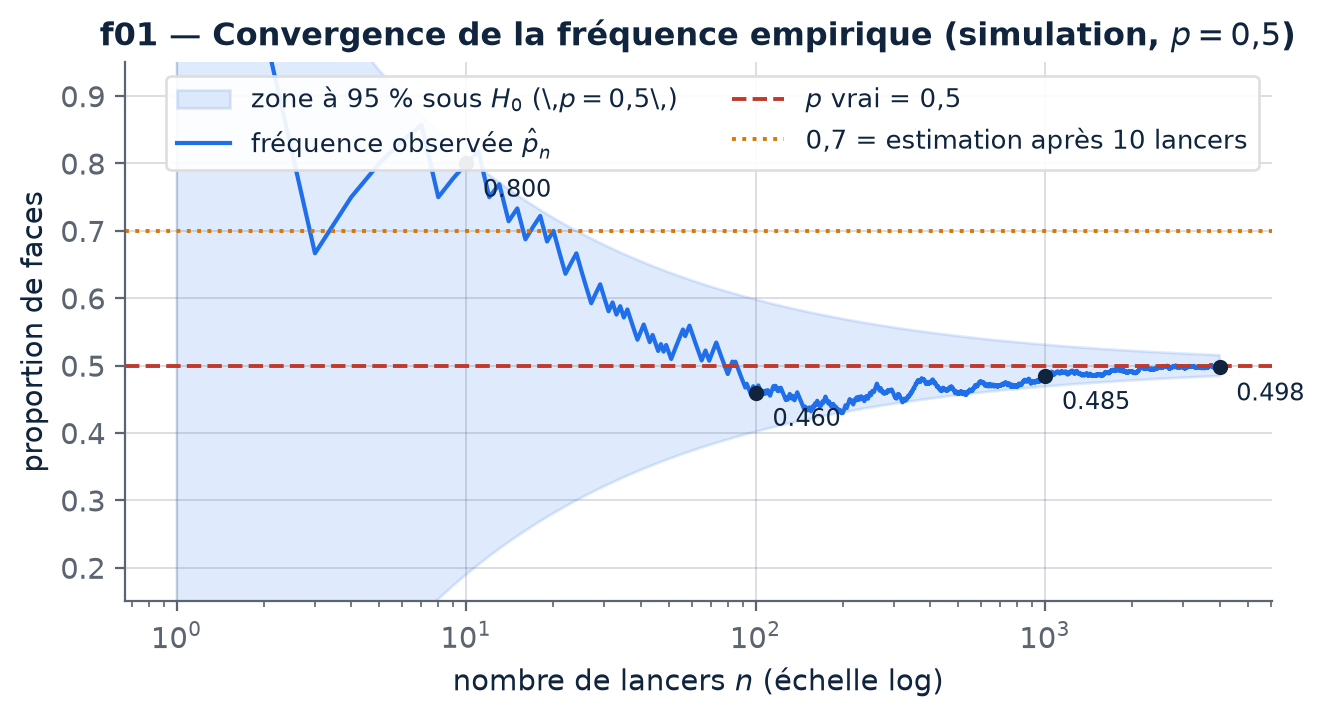
\includegraphics[width=.86\textwidth]{f01_convergence_frequence.png}
\end{center}
\end{frame}

% [split]
\begin{frame}{Ce que dit une fréquence, et ce qu'elle ne dit pas}

\vspace{-1mm}
\begin{columns}[t]
\begin{column}{0.54\textwidth}
\begin{ebox}[Lecture des données simulées]
Après 10 lancers on observe $\hat p = $ \textbf{0,80}. Après 4000 lancers : \textbf{0,498}.
Le fréquentiste conclut : \emph{« la fréquence converge vers $p$ ; la valeur
0,80 n'est qu'une fluctuation »} — mais il ne peut pas parler de $P(0{,}45 < p < 0{,}55)$\dots
\end{ebox}
\end{column}
\begin{column}{0.42\textwidth}
\begin{wbox}[Le piège fréquentiste]
\begin{itemize}
  \item $p$ n'est pas une variable : aucune probabilité ne lui est attachée.
  \item L'IC à 95 \% est \textbf{un long terme théorique}, pas la confiance dans
        \emph{cet} intervalle calculé.
  \item Aucun moyen d'injecter le fait que la pièce semble équilibrée \textit{a priori}.
\end{itemize}
\end{wbox}
\end{column}
\end{columns}
\end{frame}

% ---------------------------------------------------------------- 11
\begin{frame}{La probabilité comme état de connaissance}
\begin{kbox}[Postulat bayésien]
Une probabilité est une \textbf{appréciation de plausibilité par un agent} cohérent.
Deux agents avec des informations différentes \emph{doivent} avoir des probabilités
différentes — et c'est une force, à condition de dire lesquelles.
\end{kbox}
\vspace{2mm}
\begin{columns}[t]
\begin{column}{0.48\textwidth}
\begin{ebox}[Exemple 1 — question piégée]
« Quelle est la probabilité que la Chine soit le premier pays à poser un humain sur Mars ? »
\vspace{1mm}
\footnotesize Il n'y a pas de « fréquence de long terme » : l'événement est unique.
Pourtant on sait raisonner, comparer, mettre à jour.
\end{ebox}
\end{column}
\begin{column}{0.48\textwidth}
\begin{ebox}[Exemple 2 — l'ordre]
« Ce patient a survécu 3 mois au traitement. »
\vspace{1mm}
\footnotesize Le bayésien peut arrêter l'essai quand les données le justifient
(interprétation \textit{conditionnelle} aux données observées),
sans gonfler artificiellement le risque de première espèce.
\end{ebox}
\end{column}
\end{columns}
\vspace{1.5mm}
\begin{tcolorbox}[colback=byCyan!8,colframe=byCyan,arc=2mm,width=.95\textwidth]
\small\centering
\textbf{Conséquence pratique :} la conclusion bayésienne s'énonce
\textbf{conditionnellement aux données réellement observées} — pas sur des
répétitions imaginaires de l'expérience.
\end{tcolorbox}
\end{frame}

% ---------------------------------------------------------------- 12
\begin{frame}{Mise à jour séquentielle : le cœur du raisonnement}
\begin{ebox}[Principe]
Le posterior d'aujourd'hui devient le prior de demain :
$p(\theta \given y_1, y_2) \neq$ refaire tout le calcul, mais
$p(\theta \given y_1, y_2) \propto p(\theta) \, p(y_1 \given \theta) \, p(y_2 \given \theta)$.
L'ordre d'arrivée des données \textbf{ne change pas} le résultat.
\end{ebox}
\vspace{1mm}
\begin{center}
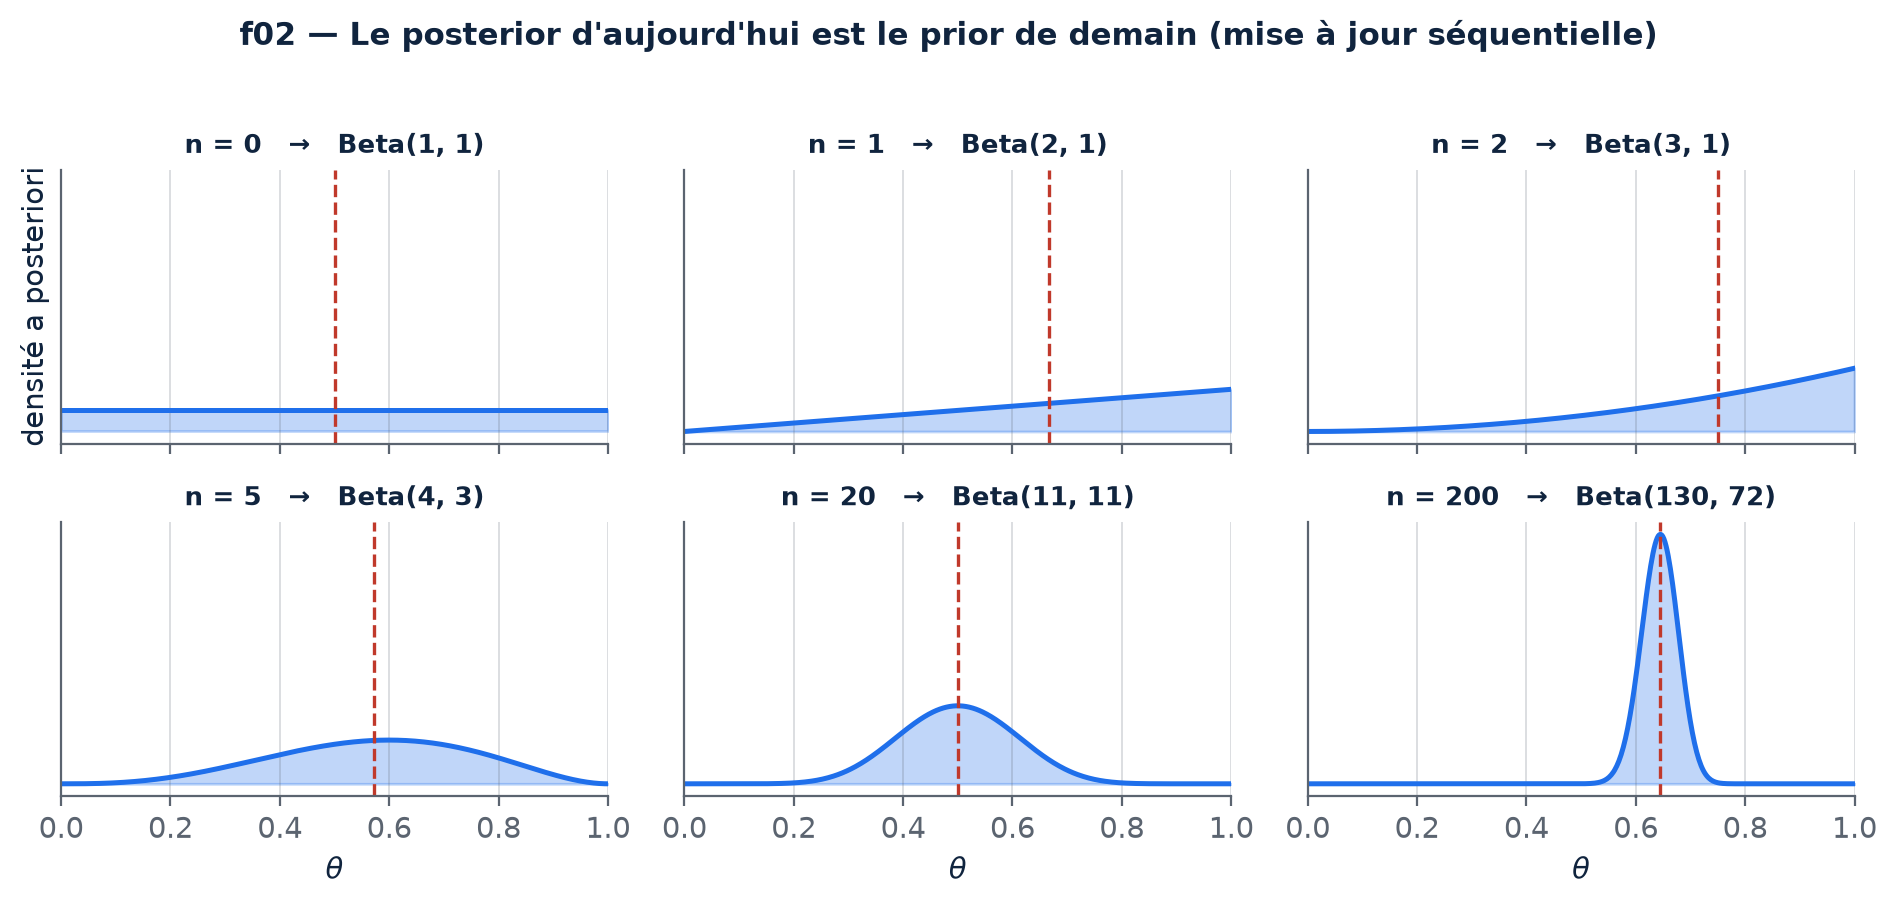
\includegraphics[width=.82\textwidth]{f02_beta_updating.png}
\end{center}
\vspace{-1mm}
\centering\footnotesize
Simulation réelle : 200 lancers d'une pièce biaisée ($p = 0{,}65$), prior Beta$(1,1)$.
La dispersion se resserre comme $1/\sqrt{n}$ : c'est la \emph{vitesse d'apprentissage}.
\end{frame}
% ---------------------------------------------------------------- 13
\begin{frame}{Vocabulaire : quatre objets, un raisonnement}
\begin{center}
{\setlength{\tabcolsep}{3pt}\begin{tabular}{@{}p{2.0cm}p{2.5cm}p{4.2cm}p{4.3cm}@{}}
\toprule
\textbf{Objet} & \textbf{Notation} & \textbf{Interprétation} & \textbf{Exemple (pièce biaisée)} \\
\midrule
A priori & $p(\theta)$ & ce que l'on croit \emph{avant} les données &
Beta$(2,2)$ : « la pièce est plausiblement équilibrée » \\[2mm]
Vraisemblance & $p(y \given \theta)$ & probabilité des données \emph{si} le paramètre valait $\theta$ &
Bin$\big(10, \theta\big)$ : 7 faces sur 10 \\[2mm]
A posteriori & $p(\theta \given y)$ & la croyance \emph{après} les données &
Beta$(9,5)$ : centré sur 0,64 \\[2mm]
Prédictive & $p(\tilde y \given y)$ & ce qu'on attend de la prochaine observation &
$P(\text{face}) = \int \theta\, p(\theta \given y)\,\mathrm{d}\theta = 0{,}643$ \\
\bottomrule
\end{tabular}}
\end{center}
\vspace{1mm}
\begin{kbox}[La règle d'or]
Le prior est \textbf{ce qu'on met sur la table} ; le posterior est
\textbf{ce qui en reste après avoir vu les données}. Rien ne se perd, tout se met à jour.
\end{kbox}
\end{frame}

% ---------------------------------------------------------------- 14
\begin{frame}{Exemple fondateur : la pièce truquée --- l'énoncé}
\begin{ebox}[Énoncé]
On lance 10 fois une pièce et on obtient \textbf{7 faces}.
\begin{itemize}
  \item Paramètre : $\theta = P(\text{face}) \in [0,1]$
  \item Prior : $\theta \sim \mathrm{Beta}(1,1)$ (uniforme)
  \item Vraisemblance : $y \given \theta \sim \mathrm{Bin}(10, \theta)$
\end{itemize}
\vspace{1mm}
\textbf{Questions}
\begin{enumerate}
  \item Forme du posterior ?
  \item Valeur centrale ?
  \item Intervalle de crédibilité à 95 \% ?
  \item $P(\theta > 0{,}5 \given y)$ ?
\end{enumerate}
\end{ebox}
\end{frame}

% [split]
\begin{frame}{Exemple fondateur : la pièce truquée --- le posterior}
\begin{center}
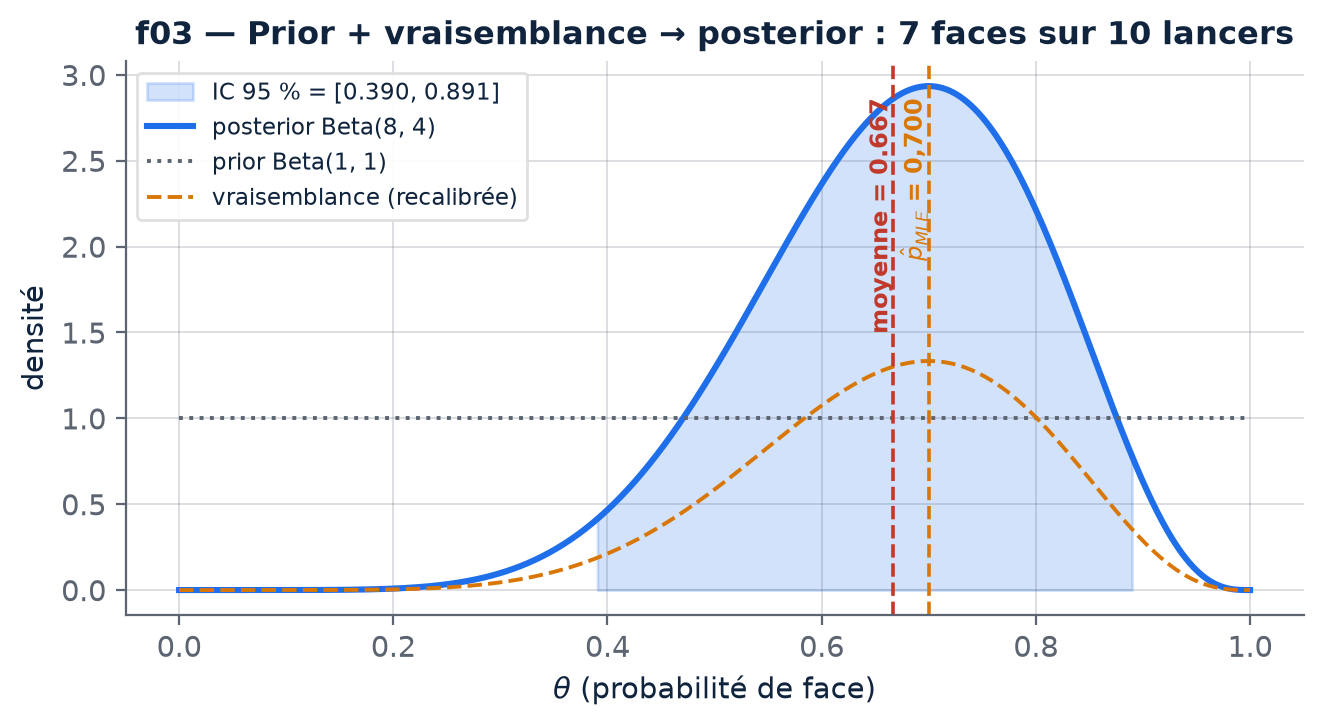
\includegraphics[width=.86\textwidth]{f03_piece_posterior.png}
\end{center}
\end{frame}

% [split]
\begin{frame}{Exemple fondateur : la pièce truquée --- le posterior}

\vspace{-1mm}
\begin{solbox}[Résultats calculés (script \file{src/fig\_ch1.py}, exécuté)]
\centering\small
posterior $\mathrm{Beta}(8,4)$ \quad|\quad moyenne $0{,}667$ \quad|\quad mode $0{,}700$
\quad|\quad IC 95 \% $[0{,}390 \,;\, 0{,}891]$ \quad|\quad $P(\theta > 0{,}5 \given y) = 0{,}887$
\end{solbox}
\end{frame}

% ---------------------------------------------------------------- 15
% [suite]
\begin{frame}{Comment lire un résultat bayésien}
\begin{columns}[t]
\begin{column}{0.5\textwidth}
\begin{kbox}[Trois nombres]
\begin{itemize}
  \item \textbf{Moyenne a posteriori} $0{,}667$ : minimise l'erreur quadratique,
        c'est l'estimateur par défaut.
  \item \textbf{Médiane} : robuste, sert au calcul du HDI.
  \item \textbf{Mode (MAP)} $0{,}700$ : coïncide ici avec le maximum de vraisemblance.
        Avec un prior asymétrique, il s'en écarte — c'est le \emph{shrinkage}.
\end{itemize}
\end{kbox}
\end{column}
\begin{column}{0.47\textwidth}
\begin{solbox}[Intervalle de crédibilité 95 \%]
$[0{,}390 \,;\, 0{,}891]$

\vspace{1.5mm}
\small « Il y a 95 \% de chance que la vraie probabilité de face soit dans cet intervalle,
\textbf{compte tenu du prior et des 7 faces observées}. »

\vspace{1.5mm}
Variante HDI (le plus court des intervalles de masse 0,95) : $[0{,}412 \,;\, 0{,}906]$ ---
légèrement plus court que l'intervalle à queues égales.
\end{solbox}
\end{column}
\end{columns}
\vspace{1mm}
\begin{ebox}[Effet mesurable du prior, mêmes données]
Avec $\theta \sim \mathrm{Beta}(2,2)$ au lieu de Beta$(1,1)$ : posterior $\mathrm{Beta}(9,5)$,
moyenne $0{,}643$, IC 95 \% $[0{,}386 \,;\, 0{,}861]$.
Le prior a ramené la croyance de 0,667 vers 0,643 : c'est le \textbf{\textit{shrinkage}}.
\end{ebox}
\vspace{1mm}
\end{frame}

% [suite]
\begin{frame}{Comment lire un résultat bayésien (suite)}
\begin{wbox}[À ne jamais écrire]
\nok{} « Il y a 95 \% de chance que la vraie valeur soit dans \emph{l'intervalle de confiance
fréquentiste} » \;; \;
\nok{} « $p(\theta) = 0{,}667$ est la probabilité que $\theta$ vaille exactement 0,667 »
(probabilité d'un point : nulle pour une loi continue).
\end{wbox}
\end{frame}

% ---------------------------------------------------------------- 16
\begin{frame}{Animation : mise à jour, observation après observation}
% [rogna]
\small
\begin{columns}[t]
\begin{column}{0.56\textwidth}
\begin{center}
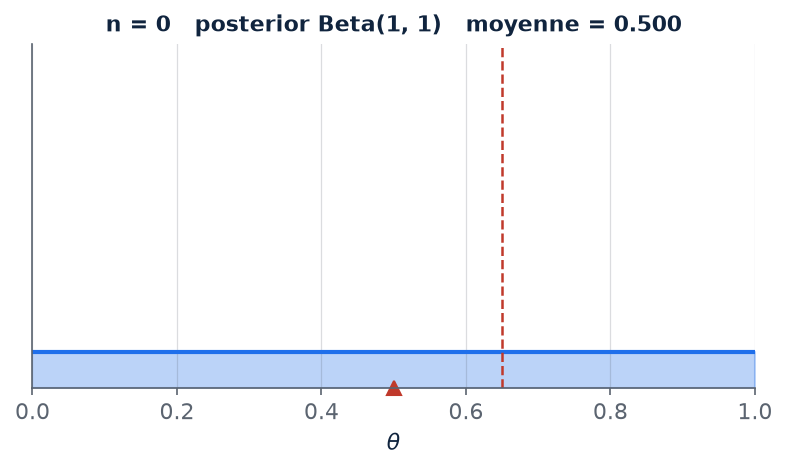
\includegraphics[width=\textwidth]{f04_frames/frame-0.png}
\end{center}
\vspace{-2mm}
\centering\footnotesize
\begin{tabular}{@{}llll@{}}
\toprule
$n$ & faces observées & posterior & moyenne \\
\midrule
0 (prior) & 0 & Beta$(1,1)$ & 0,500 \\
1 & 1 & Beta$(2,1)$ & 0,667 \\
5 & 5 & Beta$(6,1)$ & 0,857 \\
20 & 16 & Beta$(17,5)$ & 0,773 \\
200 & 121 & Beta$(122,80)$ & 0,604 \\
\bottomrule
\end{tabular}
\end{column}
\begin{column}{0.42\textwidth}
\begin{abox}[À faire devant la classe]
Ouvrir \file{notebooks/TP1\_mise\_a\_jour\_\allowbreak bayesienne.ipynb} et rejouer l'animation
($\alpha$, $\beta$ modifiables).

\vspace{1.5mm}
\textbf{Question :} à partir de quel $n$ une observation supplémentaire
déplace-t-elle la moyenne de moins de 0,005 ?
\end{abox}
\vspace{1mm}
\begin{ebox}[Réponse (calculée)]
Pour la réalisation simulée à $n = 200$, l'écart-type du posterior vaut $0{,}034$
et la moyenne ne bouge que de $\approx 0{,}002$ par nouvelle observation.
$5$ faces sur les $5$ premiers lancers donnaient 0,857 : \textbf{le petit échantillon
est extrême}, l'information ne s'achète pas, elle s'accumule en $1/\sqrt{n}$.
\end{ebox}
\end{column}
\end{columns}
\end{frame}

% ---------------------------------------------------------------- 17
% [split]
\begin{frame}{Application : sondage électoral}
\begin{center}
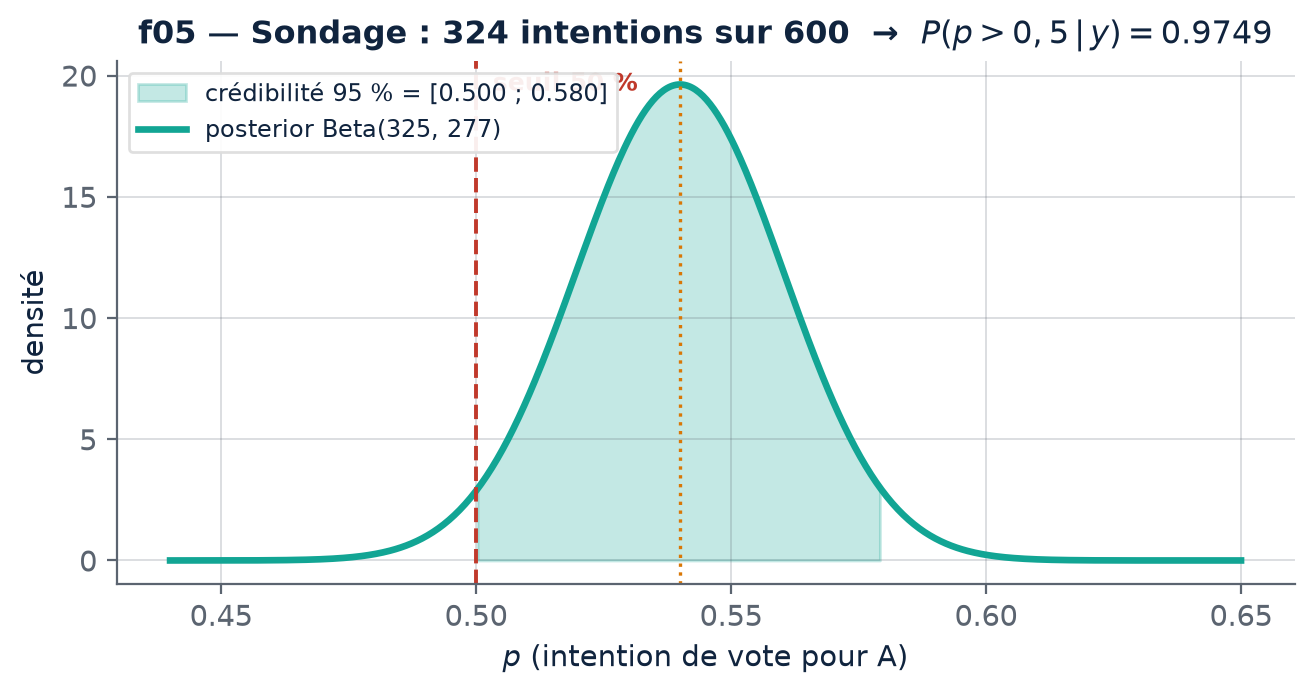
\includegraphics[width=\textwidth]{f05_sondage_posterior.png}
\end{center}
\end{frame}

% [split]
% [suite5]
\begin{frame}{Application : sondage électoral}
\begin{columns}[t]
\begin{column}{0.48\textwidth}
\begin{ebox}[Données]
$n = 600$ personnes interrogées, \textbf{324} intentions de vote pour A (54,0 \%).
Prior Beta$(1,1)$.
\end{ebox}
\begin{solbox}[Ce qu'on peut dire]
\begin{itemize}
  \item Posterior : $\mathrm{Beta}(325, 277)$, moyenne $0{,}540$
  \item Crédibilité 95 \% : $[0{,}500 \,;\, 0{,}580]$
  \item \textbf{$P(p > 0{,}5 \given y) = 0{,}975$}
  \item $P(p > 0{,}52) = 0{,}836$ \quad (intérêt : la marge d'un second tour)
  \item $P(p > 0{,}55) = 0{,}310$ \quad (le candidat est loin d'être certain de passer)
\end{itemize}
\end{solbox}
\end{column}
\end{columns}
\end{frame}

% [suite5]
\begin{frame}{Application : sondage électoral (suite)}
\begin{kbox}[L'avantage décisif]
Le fréquentiste donne $[0{,}50 \,;\, 0{,}58]$ mais ne peut pas répondre à
« le candidat A est-il \emph{probablement} au-dessus de 50 \% ? ».
Le bayésien répond : \textbf{97,5 \%}.
\end{kbox}
\end{frame}

% ---------------------------------------------------------------- 18
\begin{frame}{Pièges de lecture des intervalles}
\begin{columns}[t]
\begin{column}{0.49\textwidth}
\begin{wbox}[Intervalle de confiance fréquentiste]
\begin{itemize}
  \item Construit sur la variabilité de $\hat p$.
  \item \textbf{Ce dont on est sûr :} si l'on répétait l'étude un très grand nombre de fois,
        alors 95 \% des intervalles ainsi construits contiendraient $p$.
  \item \textbf{Ce dont on n'est pas sûr :} que \emph{cet} intervalle contienne $p$.
  \item Il ne peut pas devenir plus étroit quand on dispose d'information externe
        \emph{à moins} de changer la méthode.
\end{itemize}
\end{wbox}
\end{column}
\begin{column}{0.49\textwidth}
\begin{solbox}[Intervalle de crédibilité bayésien]
\begin{itemize}
  \item Construit sur la variabilité de $\theta$.
  \item \textbf{Ce dont on est sûr :} $P(\theta \in [a,b] \given y) = 0{,}95$.
  \item Il \textbf{rétrécit} mécaniquement si l'on ajoute de l'information externe
        justifiée (les priors conjugués du chapitre 2).
  \item Variante HDI : l'intervalle \emph{le plus court} de masse 0,95
        (chapitre 3, slide sur HDI contre queue égale).
\end{itemize}
\end{solbox}
\end{column}
\end{columns}
\vspace{1mm}
\centering\small
Les deux intervalles se ressemblent numériquement quand $n$ est grand —
ils \textbf{ne racontent pas la même chose}.
\end{frame}
% ---------------------------------------------------------------- 19
\begin{frame}{Le théorème de Bayes}
\begin{columns}[t]
\begin{column}{0.50\textwidth}
\begin{tcolorbox}[enhanced,colback=byDeep!6,colframe=byBlue,arc=2mm,
   boxrule=1pt,left=2mm,right=2mm,top=2mm,bottom=2mm]
\centering\large
\[
\underbrace{p(\theta \given y)}_{\text{a posteriori}}
\;=\;
\frac{\overbrace{p(y \given \theta)}^{\text{vraisemblance}}\;
      \overbrace{p(\theta)}^{\text{a priori}}}
     {\underbrace{\int p(y \given \theta')\,p(\theta')\,\mathrm{d}\theta'}_{\text{constante de normalisation}}}
\]
\end{tcolorbox}
\vspace{1mm}
\centering\small Forme proportionnelle, celle qu'on utilise en pratique :
\[\boxed{\;p(\theta \given y) \;\propto\; p(y \given \theta)\,p(\theta)\;}\]
\end{column}
\begin{column}{0.48\textwidth}
\begin{kbox}[Pourquoi c'est vrai]
Par définition de la probabilité conditionnelle :
\[
p(\theta \given y) = \frac{p(\theta, y)}{p(y)}
= \frac{p(y \given \theta)\,p(\theta)}{p(y)}
\]
et $p(y) = \int p(y \given \theta)p(\theta)\,\mathrm{d}\theta$
ne dépend \textbf{pas} de $\theta$.
\end{kbox}
\begin{wbox}[Le mot qui change tout]
L'intégrale du dénominateur est la \textbf{vraisemblance marginale}
$p(y)$ : c'est \emph{elle} qui décidera du facteur de Bayes et de la comparaison
de modèles (chapitre 4). Ici, on peut l'ignorer grâce à la proportionnalité.
\end{wbox}
\end{column}
\end{columns}
\end{frame}

% ---------------------------------------------------------------- 20
\begin{frame}{Démonstration pas à pas (3 lignes)}
\begin{abox}[On reprend la pièce truquée : prior Beta$(1,1)$, 7 faces sur 10]
\[
\begin{aligned}
\text{1. A priori}\quad & p(\theta) = \frac{\Gamma(2)}{\Gamma(1)\Gamma(1)}\theta^{0}(1-\theta)^{0} = 1 \\[1.5mm]
\text{2. Vraisemblance}\quad & p(y \given \theta) = \binom{10}{7}\theta^{7}(1-\theta)^{3} \\[1.5mm]
\text{3. Produit}\quad & p(\theta \given y) \propto \underbrace{\theta^{7}(1-\theta)^{3}}_{\text{le noyau seulement}}
\end{aligned}
\]
\end{abox}
\vspace{1mm}
\begin{solbox}[Reconnaître un noyau connu]
La forme $\theta^{7}(1-\theta)^{3}$ est le noyau d'une loi Beta de paramètres
$a-1 = 7$ et $b-1 = 3$, donc $a = 8$, $b = 4$ :
\[
p(\theta \given y) = \mathrm{Beta}(8,4) = \frac{\Gamma(12)}{\Gamma(8)\Gamma(4)}\theta^{7}(1-\theta)^{3}
\]
\textbf{La constante de normalisation n'a jamais eu besoin d'être calculée} : on l'a
retrouvée en reconnaissant le noyau. C'est le mécanisme de la conjugaison.
\end{solbox}
\end{frame}

% ---------------------------------------------------------------- 21
\begin{frame}{Bayes en quatre mots et en continu}
% [rogna]
\small
\begin{columns}[t]
\begin{column}{0.48\textwidth}
\begin{kbox}[Cas discret : la version de base]
\[
P(H \given E) = \frac{P(E \given H)\,P(H)}{P(E)}
\]
\begin{itemize}
  \item $H$ : hypothèse (malade, spam, modèle)
  \item $E$ : évidence (test positif, mot « gain »)
  \item $P(H)$ : croyance \emph{avant}
  \item $P(H \given E)$ : croyance \emph{après}
\end{itemize}
\end{kbox}
\begin{ebox}[Cotes, plus commode]
\[
\underbrace{\frac{P(H \given E)}{P(\bar H \given E)}}_{\text{cotes post.}}
=
\underbrace{\frac{P(H)}{P(\bar H)}}_{\text{cotes pri.}}
\times
\underbrace{\frac{P(E \given H)}{P(E \given \bar H)}}_{\text{rapport de vraisemblance}}
\]
Avec le spam : $0{,}25 \times 12 = 3 \Rightarrow P = 3/4 = 0{,}75$.
\end{ebox}
\end{column}
\begin{column}{0.48\textwidth}
\begin{ebox}[Cas continu : le paramètre]
\[
p(\theta \given y_1, \dots, y_n) \propto p(\theta)\prod_{i=1}^{n} p(y_i \given \theta)
\]
\begin{itemize}
  \item $\theta \in \R^d$ : paramètre (vecteur)
  \item $p(\theta)$ : densité a priori
  \item l'\textbf{i.i.d.} transforme le produit en somme de log
\end{itemize}
\end{ebox}
\begin{wbox}[Trois confusions classiques]
\begin{itemize}
  \item $p(\theta \given y) \neq p(y \given \theta)$ : les deux ne sont
        \textbf{pas} symétriques, la seconde est la vraisemblance.
  \item Une densité peut dépasser 1 : seule l'aire vaut 1.
  \item Le posterior \emph{dépend} du prior.
\end{itemize}
\end{wbox}
\end{column}
\end{columns}
\end{frame}

% ---------------------------------------------------------------- 22
\begin{frame}{Exercice guidé 1 --- détection de spam (10 min) --- l'énoncé}
\begin{ebox}[Énoncé]
Un filtre doit classer un courriel. On sait que :
\begin{itemize}
  \item 20 \% des courriels reçus sont des spams : $P(S) = 0{,}20$
  \item le mot « gain » apparaît dans 60 \% des spams : $P(G \given S) = 0{,}60$
  \item il apparaît dans 5 \% des courriels légitimes : $P(G \given \bar S) = 0{,}05$
\end{itemize}
\vspace{1.5mm}
\noindent\textbf{Question :} le mot « gain » est présent. Quelle est la probabilité
que ce courriel soit un spam ?
\end{ebox}
\vspace{1mm}
\begin{abox}[Question bonus (celle qui fait réfléchir)]
Et si « gain » apparaît \textbf{deux fois} ? \textbf{Quatre fois} ?
Quelle hypothèse êtes-vous obligé de faire ?
\end{abox}
\end{frame}

\begin{frame}{Exercice guidé 1 --- détection de spam}
\begin{center}
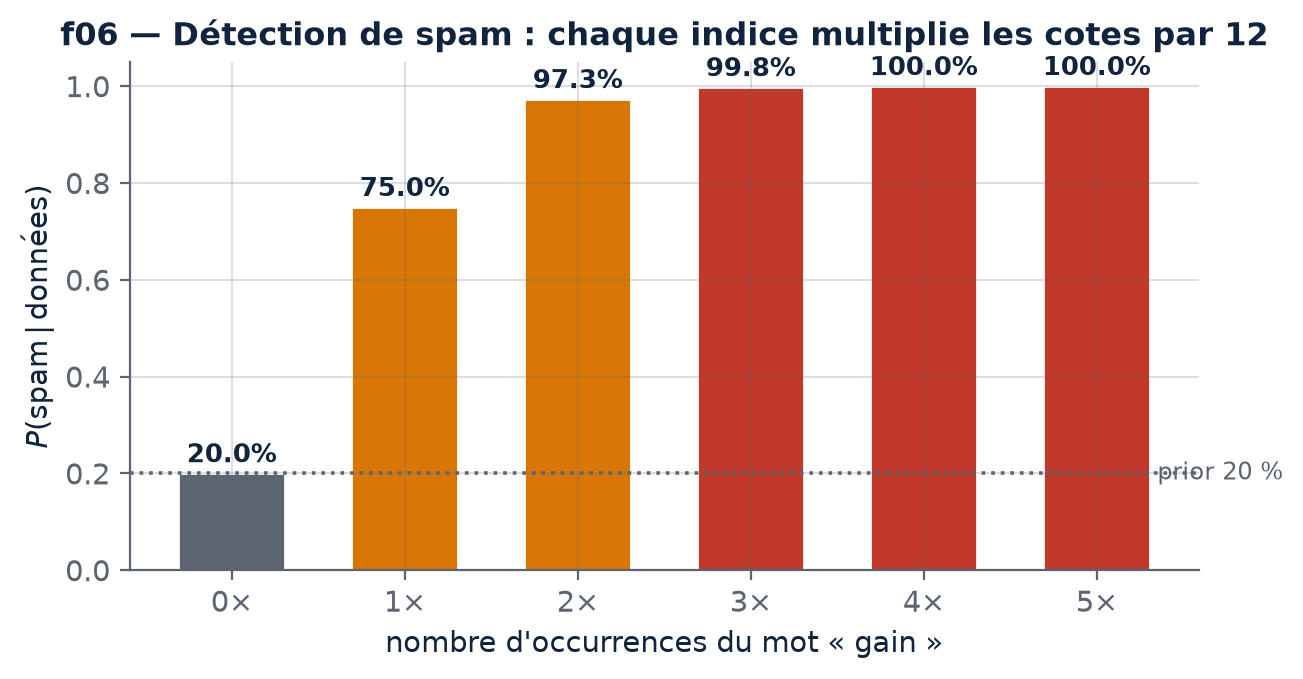
\includegraphics[width=.88\textwidth]{f06_spam.png}
\end{center}
\end{frame}

% ---------------------------------------------------------------- 23
\begin{frame}{Exercice guidé 1 — solution détaillée}
% [rogna]
\small
\begin{columns}[t]
\begin{column}{0.52\textwidth}
\begin{solbox}[Dénominateur d'abord]
\[
\begin{aligned}
P(G) &= P(G \given S)P(S) + P(G \given \bar S)P(\bar S)\\
     &= 0{,}60 \times 0{,}20 + 0{,}05 \times 0{,}80\\
     &= 0{,}12 + 0{,}04 = 0{,}16
\end{aligned}
\]
puis
\[
P(S \given G) = \frac{0{,}60 \times 0{,}20}{0{,}16} = 0{,}75
\]
Le score a été multiplié par 3 : les cotes passent de $1/4$ à $3/1$.
\end{solbox}
\end{column}
\begin{column}{0.46\textwidth}
\begin{ebox}[Occurrences répétées]
En supposant les occurrences \textbf{conditionnellement indépendantes} :
\[
P(S \given 2G) = \frac{0{,}60^2 \times 0{,}20}{0{,}60^2 \times 0{,}20 + 0{,}05^2 \times 0{,}80}
\]
\centering
\begin{tabular}{@{}lll@{}}
\toprule
Occurrences & Cotes & $P(S \given \cdot)$ \\
\midrule
0 & $0{,}25$ & 0,200 \\
1 & $3{,}0$ & \textbf{0,750} \\
2 & $36{,}0$ & \textbf{0,973} \\
3 & $432{,}0$ & \textbf{0,9977} \\
\bottomrule
\end{tabular}
\end{ebox}
\end{column}
\end{columns}
\vspace{1mm}
\begin{wbox}[Correction d'une erreur répandue]
On lit souvent « 2 occurrences $\Rightarrow$ 90 \% ». C'est faux : le calcul exact donne
\textbf{97,3 \%} ($0{,}25 \times 12^2 = 36$, soit $36/37$). Le facteur de Bayes se multiplie,
il ne s'additionne pas.
\end{wbox}
\end{frame}

% ---------------------------------------------------------------- 24
\begin{frame}{Quiz 2 — application directe}
\begin{qbox}[Question 2 -- Facteur 12]
Un filtre bayésien part d'un prior $P(S) = 0{,}20$ et traite chaque indice
indépendant comme un rapport de vraisemblance de 12.
\vspace{2mm}
Il faut dépasser 99 \% de certitude pour bloquer sans revue humaine.
Combien d'indices faut-il au minimum ?
\vspace{2mm}
\begin{enumerate}
  \item[(A)] 2 \quad \item[(B)] 3 \quad \item[(C)] 4 \quad \item[(D)] 6
\end{enumerate}
\vspace{2mm}
\textbf{Réponse : (B)} --- les cotes valent $0{,}25 \times 12^k$ ;
$k = 3$ donne 432, soit $0{,}9977 > 0{,}99$. Avec $k = 2$ on plafonne à 0,973.
\end{qbox}
\vspace{1.5mm}
\begin{kbox}[Ce que ce petit calcul enseigne]
La \textbf{mise à jour séquentielle} est une addition de log-cotes :
$\log(\text{cotes post.}) = \log(\text{cotes pri.}) + \sum_k \log(\text{LR}_k)$.
C'est exactement l'architecture d'un Naive Bayes, et c'est la raison pour laquelle
il tient sur un téléphone.
\end{kbox}
\end{frame}

% ---------------------------------------------------------------- 25
\begin{frame}{Exercice guidé 2 — le test COVID (10 min)}
\begin{columns}[t]
\begin{column}{0.47\textwidth}
\begin{ebox}[Énoncé]
Un test antigénique a
\begin{itemize}
  \item sensibilité $P(T^+ \given M) = 0{,}95$
  \item spécificité $P(T^- \given \bar M) = 0{,}98$
\end{itemize}
On teste une personne tirée au hasard dans une population où la prévalence est
de \textbf{5 \%}.
\vspace{1.5mm}
\textbf{Question :} le test est positif.
Quelle est la probabilité qu'elle soit réellement malade ?
\vspace{1.5mm}

\noindent\textcolor{byBlue}{\textbf{Indice :}} commencez par compter sur 1000 personnes.
\end{ebox}
\end{column}
\begin{column}{0.51\textwidth}
\begin{solbox}[Résolution en arbre]
Sur 1000 personnes :
\begin{itemize}
  \item 50 malades : $50 \times 0{,}95 = 47{,}5$ positifs
  \item 950 saines : $950 \times 0{,}02 = 19$ faux positifs
\end{itemize}
\[
P(M \given T^+) = \frac{47{,}5}{47{,}5 + 19} = \frac{47{,}5}{66{,}5} = \mathbf{0{,}714}
\]
\centering\footnotesize
Même sensibilité, même spécificité : la réponse dépend entièrement du contexte.
\end{solbox}
\end{column}
\end{columns}
\end{frame}

% ---------------------------------------------------------------- 26
% [split]
\begin{frame}{Le même test, six vérités différentes}
\begin{center}
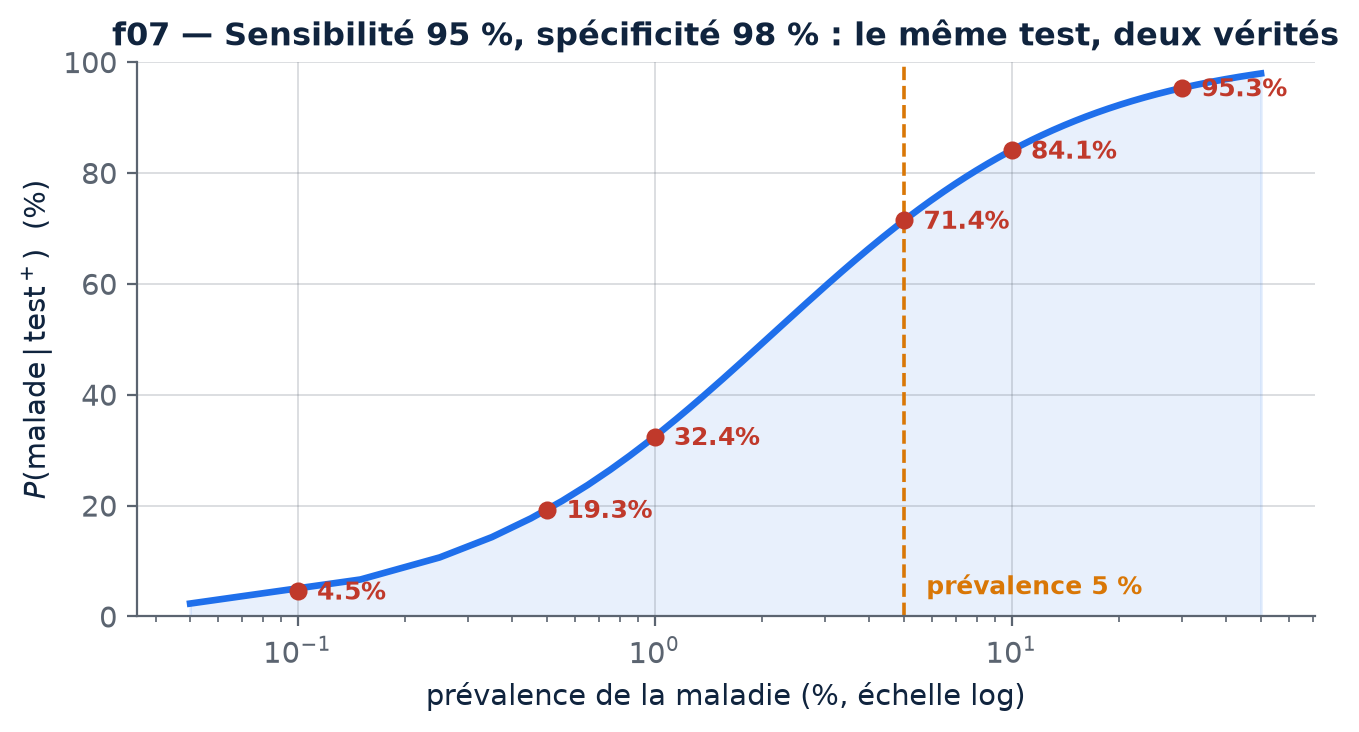
\includegraphics[width=.86\textwidth]{f07_covid_ppv.png}
\end{center}
\end{frame}

% [split]
\begin{frame}{Le même test, six vérités différentes}

\vspace{-1mm}
\begin{columns}[t]
\begin{column}{0.62\textwidth}
\begin{tabular}{@{}lcccccc@{}}
\toprule
Prévalence & 0,1 \% & 0,5 \% & 1 \% & 5 \% & 10 \% & 30 \% \\
\midrule
$P(M \given T^+)$ & 4,5 \% & 19,3 \% & 32,4 \% & \textbf{71,4 \%} & 84,1 \% & 95,3 \% \\
\bottomrule
\end{tabular}
\vspace{1.5mm}

\small Toutes ces valeurs sortent du calcul exécuté dans \file{src/fig\_ch1.py}.
\end{column}
\begin{column}{0.36\textwidth}
\begin{kbox}[Le cœur du cours]
La prévalence \textbf{est} un prior. La formule de Bayes n'est pas une recette de
calcul : c'est la déclaration explicite qu'\emph{une conclusion dépend de ce qu'on
croyait avant de mesurer}.
\end{kbox}
\end{column}
\end{columns}
\end{frame}
% ---------------------------------------------------------------- 27
% [suite5]
\begin{frame}[fragile]{Boîte à outils : la fonction qui fait tout}
% [rogna]
\small
\begin{columns}[t]
\begin{column}{0.53\textwidth}
\begin{codebox}[bayes.py — version minimale et générale]
\begin{lstlisting}
import numpy as np
from scipy import stats

def posterior_discret(prior_grid, prior_pdf, vraisemblance, y):
    """Posterior sur une grille : suffit des que theta est
    de dimension 1 ou 2. Aucune formule close requise."""
    post = prior_pdf(prior_grid) * vraisemblance(prior_grid, y)
    post /= np.trapezoid(post, prior_grid)     # normalisation
    return post

def proba(prior_grid, post, seuil):
    """P(theta > seuil | y) : LA question a laquelle le
    frequentiste ne peut pas repondre."""
    m = prior_grid > seuil
    return np.trapezoid(post[m], prior_grid[m])

def intervale_credibilite(prior_grid, post, niveau=0.95):
    c = np.cumsum(post) / post.sum()
    lo = prior_grid[np.searchsorted(c, (1 - niveau) / 2)]
    hi = prior_grid[np.searchsorted(c, 1 - (1 - niveau) / 2)]
    return lo, hi
\end{lstlisting}
\end{codebox}
\end{column}
\begin{column}{0.45\textwidth}
\begin{kbox}[Trois fonctions, tout le chapitre]
\begin{itemize}
  \item \textbf{grille $+$ normalisation} : la méthode universelle quand
        aucune conjugaison n'est disponible ;
  \item \textbf{proba dépassant un seuil} : la question décisionnelle ;
  \item \textbf{intervalle de crédibilité} : la synthèse de l'incertitude.
\end{itemize}
\end{kbox}
\end{column}
\end{columns}
\end{frame}

% [suite5]
\begin{frame}{Boîte à outils : la fonction qui fait tout (suite)}
\begin{wbox}[Quand la grille ne suffit plus]
En dimension $d$, une grille coûte $n^d$ points : impossible au-delà de
$d \approx 3$. C'est \textbf{exactement} le mur qui a motivé les méthodes MCMC
(chapitre 5).
\end{wbox}
\end{frame}

% ---------------------------------------------------------------- 28
\begin{frame}{Ce qui change quand le paramètre devient continu}
\begin{columns}[t]
\begin{column}{0.49\textwidth}
\begin{ebox}[Cas continu, exemple complet]
Mesures répétées d'une grandeur physique, $y_i \sim \N(\mu, \sigma^2)$ avec
$\sigma$ connu :
\[
\begin{aligned}
p(\mu) &= \N(\mu_0, \tau_0^2) \quad\text{(prior)}\\
p(y \given \mu) &\propto \prod_{i=1}^n e^{-\frac{(y_i-\mu)^2}{2\sigma^2}}\\
&\propto e^{-\frac{n(\bar y - \mu)^2}{2\sigma^2}}
\end{aligned}
\]
Le posterior est encore \textbf{normal} : $\N(\mu_n, \tau_n^2)$ avec
\[
\frac{1}{\tau_n^2} = \frac{1}{\tau_0^2} + \frac{n}{\sigma^2}
\]
\end{ebox}
\end{column}
\begin{column}{0.49\textwidth}
\begin{kbox}[Lecture : la précision s'additionne]
Ce n'est pas $\mu$ qui s'additionne, c'est l'\textbf{information}
$1/$variance. Le posterior est la moyenne pondérée des deux sources,
avec les poids $1/\tau_0^2$ et $n/\sigma^2$.
\vspace{1mm}
\[
\mu_n = \frac{\frac{\mu_0}{\tau_0^2}+\frac{n\bar y}{\sigma^2}}{\frac{1}{\tau_0^2}+\frac{n}{\sigma^2}}
\]
\end{kbox}
\begin{ebox}[Chiffres]
Avec $\mu_0 = 100$, $\tau_0 = 10$, $\sigma = 5$, $n = 4$, $\bar y = 92$ :
$\mu_n = 93{,}3$ et $\tau_n = 2{,}44$.
Le prior pèse encore, mais les données dominent déjà.
\end{ebox}
\end{column}
\end{columns}
\end{frame}

% ---------------------------------------------------------------- 29
% [suite]
% [suite5]
\begin{frame}{La constante de normalisation : pourquoi on l'ignore}
\begin{columns}[t]
\begin{column}{0.52\textwidth}
\begin{kbox}[Le raisonnement]
\[
p(\theta \given y) = \frac{p(y \given \theta)p(\theta)}{\underbrace{p(y)}_{\text{indépendant de }\theta}}
\]
$p(y)$ est le \emph{même nombre} pour toutes les valeurs de $\theta$ :
il \textbf{recentre} la courbe, il ne la \textbf{redessine} pas. Pour
comparer deux valeurs de $\theta$, il disparaît.
\end{kbox}
\end{column}

\begin{column}{0.46\textwidth}
\begin{wbox}[Ne l'oubliez jamais : il revient]
$p(y)$ réapparaît dans trois situations \textbf{décisives} :
\begin{itemize}
  \item \textbf{Comparer deux modèles} : c'est le facteur de Bayes
        $BF_{12} = p(y \given M_1)/p(y \given M_2)$ (chapitre 4) ;
  \item \textbf{Choisir un prior} : $p(y)$ mesure la \emph{plausibilité}
        du prior avant de voir les données (checks prédictifs a priori) ;
  \item \textbf{Modèles hiérarchiques} : il faut intégrer les effets
        latents pour évaluer la vraisemblance marginale.
\end{itemize}
\end{wbox}
\end{column}
\end{columns}
\end{frame}

% [suite5]
\begin{frame}{La constante de normalisation : pourquoi on l'ignore (suite)}
\begin{ebox}[Ordre de grandeur]
Dans l'exemple Beta-Binomial, $p(y)$ vaut exactement
$P(Y = 7)$ sous la loi prédictive a priori :
\[
p(y) = \binom{10}{7}\frac{\Gamma(2)\Gamma(11)}{\Gamma(13)} = \frac{1}{12} = 0{,}0833
\]
Le posterior $\mathrm{Beta}(8,4)$ divisé par ce facteur redonne bien une densité d'aire 1.
\end{ebox}
\end{frame}

% [suite]
\begin{frame}{La constante de normalisation : pourquoi on l'ignore (suite)}
\begin{kbox}[Règle pratique]
On travaille en \textbf{logarithme} :
$\log p(\theta \given y) = \log p(y \given \theta) + \log p(\theta) + \text{cte}$.
Toute l'inférence numérique (grilles, MCMC, VI) optimise ou échantillonne ce log-posterior.
\end{kbox}

\end{frame}

% ---------------------------------------------------------------- 30
\begin{frame}{Le mécanisme : une multiplication, pas une recette}
\begin{center}
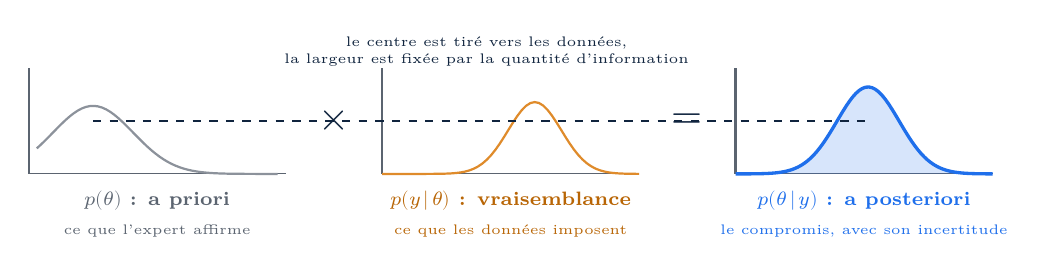
\begin{tikzpicture}[xscale=1.02,yscale=.96]
% --- prior
\draw[byGrey,thin] (-0.1,0) -- (3.1,0);
\draw[-,thick,byGrey] (-0.1,0) -- (-0.1,1.4);
\draw[byGrey!70,thick,domain=0:3,samples=60] plot (\x,{0.9*exp(-((\x-0.7)^2)/0.5)});
\node[byGrey,font=\scriptsize\bfseries] at (1.5,-0.35) {$p(\theta)$ : a priori};
\node[byGrey,font=\tiny] at (1.5,-0.75) {ce que l'expert affirme};
% --- x
\node[byDeep,font=\Large\bfseries] at (3.7,0.7) {$\times$};
% --- vraisemblance
\draw[byGrey,thin] (4.3,0) -- (7.5,0);
\draw[-,thick,byGrey] (4.3,0) -- (4.3,1.4);
\draw[byOrange!85,thick,domain=4.3:7.5,samples=60]
   plot (\x,{0.95*exp(-((\x-6.2)^2)/0.22)});
\node[byOrange!85!black,font=\scriptsize\bfseries] at (5.9,-0.35) {$p(y \given \theta)$ : vraisemblance};
\node[byOrange!85!black,font=\tiny] at (5.9,-0.75) {ce que les données imposent};
% --- =
\node[byDeep,font=\Large\bfseries] at (8.1,0.7) {$=$};
% --- posterior
\draw[byGrey,thin] (8.7,0) -- (11.9,0);
\draw[-,thick,byGrey] (8.7,0) -- (8.7,1.4);
\draw[byBlue,very thick,domain=8.7:11.9,samples=80]
   plot (\x,{1.15*exp(-((\x-10.35)^2)/0.30)});
\fill[byBlue,opacity=.18,domain=8.7:11.9,samples=80]
   (8.7,0) -- plot (\x,{1.15*exp(-((\x-10.35)^2)/0.30)}) -- (11.9,0) -- cycle;
\node[byBlue,font=\scriptsize\bfseries] at (10.3,-0.35) {$p(\theta \given y)$ : a posteriori};
\node[byBlue,font=\tiny] at (10.3,-0.75) {le compromis, avec son incertitude};
% --- annotations
\draw[byDeep,dashed,thin] (0.7,0.7) -- (10.35,0.7);
\node[byDeep,font=\tiny,align=center] at (5.6,1.62) {le centre est tiré vers les données, \\ la largeur est fixée par la quantité d'information};
\end{tikzpicture}
\end{center}
\vspace{1mm}
\begin{columns}[t]
\begin{column}{0.48\textwidth}
\begin{kbox}[Trois cas]
\begin{itemize}
  \item $\,$ prior étroit, données rares $\Rightarrow$ le prior gagne ;
  \item prior large, données nombreuses $\Rightarrow$ les données gagnent ;
  \item les deux étroits et \textbf{déplacés} $\Rightarrow$ conflit prior/données :
        \textbf{signalez-le}, ne le cachez pas.
\end{itemize}
\end{kbox}
\end{column}
\begin{column}{0.48\textwidth}
\begin{abox}[Démonstration en direct]
On rejoue la même figure avec $\alpha,\beta$ modifiables et
$n$ croissant dans le notebook
\file{TP1\_mise\_a\_jour\_\allowbreak bayesienne.ipynb} (dossier \file{notebooks/}), section 4.
\end{abox}
\end{column}
\end{columns}
\end{frame}

% ---------------------------------------------------------------- 31
\begin{frame}{Mise à jour séquentielle : la version formelle}
\begin{columns}[t]
\begin{column}{0.5\textwidth}
\begin{kbox}[Traitement par lot]
\[
p(\theta \given y_1,\dots,y_n) \propto p(\theta)\prod_{i=1}^{n}p(y_i \given \theta)
\]
\end{kbox}
\begin{kbox}[Traitement en flux (= c'est pareil)]
\[
\begin{aligned}
p(\theta \given y_1) &\propto p(\theta)\,p(y_1 \given \theta)\\
p(\theta \given y_1,y_2) &\propto p(\theta \given y_1)\,p(y_2 \given \theta)\\
&\;\;\vdots
\end{aligned}
\]
Aucune information n'est perdue : le posterior contient
\emph{toute} l'information apportée par les données déjà vues.
\end{kbox}
\end{column}
\begin{column}{0.48\textwidth}
\begin{ebox}[Conséquence majeure]
Un modèle bayésien peut être \textbf{actualisé en continu} : c'est ce qui
rend le filtrage de Kalman, les bandits bayésiens, l'arrêt anticipé des essais
cliniques et l'A/B testing séquentiel possibles \emph{sans pénalité de multiplicité}.
\end{ebox}
\begin{wbox}[Attention au raccourci]
« Le posterior suffit » n'est vrai que si le \textbf{modèle} est resté le même.
Changer de modèle (ajouter une covariable, abandonner la normalité) impose de
réévaluer le prior et la vraisemblance : le posterior d'un modèle A n'est
pas le prior d'un modèle B.
\end{wbox}
\end{column}
\end{columns}
\end{frame}

% ---------------------------------------------------------------- 32
\begin{frame}[fragile]{Exemple complet : régression linéaire bayésienne}
\begin{columns}[t]
\begin{column}{0.5\textwidth}
\begin{ebox}[Données et modèle]
12 mesures d'un rendement $y$ en fonction d'une dose $x$ (0 à 10).
\[
y_i = \beta_0 + \beta_1 x_i + \varepsilon_i, \qquad
\varepsilon_i \sim \N(0, \sigma^2)
\]
Priors \textbf{faiblement informatifs} :
\[
\beta_0 \sim \N(0, 5^2),\quad
\beta_1 \sim \N(0{,}5, 1^2),\quad
\sigma \sim \text{Demi-Normale}(2)
\]
\end{ebox}
\begin{kbox}[Pourquoi ces priors ?]
Volontairement larges : ils n'imposent rien de précis, mais ils
\textbf{empêchent des valeurs absurdes} (une pente de $10^6$). Ils disent
« je m'attends à un effet modéré, dans un ordre de grandeur raisonnable ».
\end{kbox}
\end{column}
\begin{column}{0.48\textwidth}
\begin{codebox}[PyMC — le modèle complet]
\begin{lstlisting}
with pm.Model() as modele:
    b0 = pm.Normal("b0", mu=0, sigma=5)
    b1 = pm.Normal("b1", mu=0.5, sigma=1)
    sigma = pm.HalfNormal("sigma", sigma=2)
    mu = b0 + b1 * x
    pm.Normal("y", mu=mu, sigma=sigma, observed=y)
    trace = pm.sample(draws=2000, tune=1500, chains=2)
\end{lstlisting}
\end{codebox}
\begin{abox}[Ce que l'on va lire sur le résultat]
\begin{itemize}
  \item la postérieure de chaque coefficient ;
  \item l'intervalle de crédibilité à 95 \% ;
  \item la prévision \textbf{avec} son incertitude.
\end{itemize}
\end{abox}
\end{column}
\end{columns}
\end{frame}

% ---------------------------------------------------------------- 33
% [rogna]
% [split]
\begin{frame}{Résultats réels (exécutés sur cette machine, CPU)}
\begin{center}
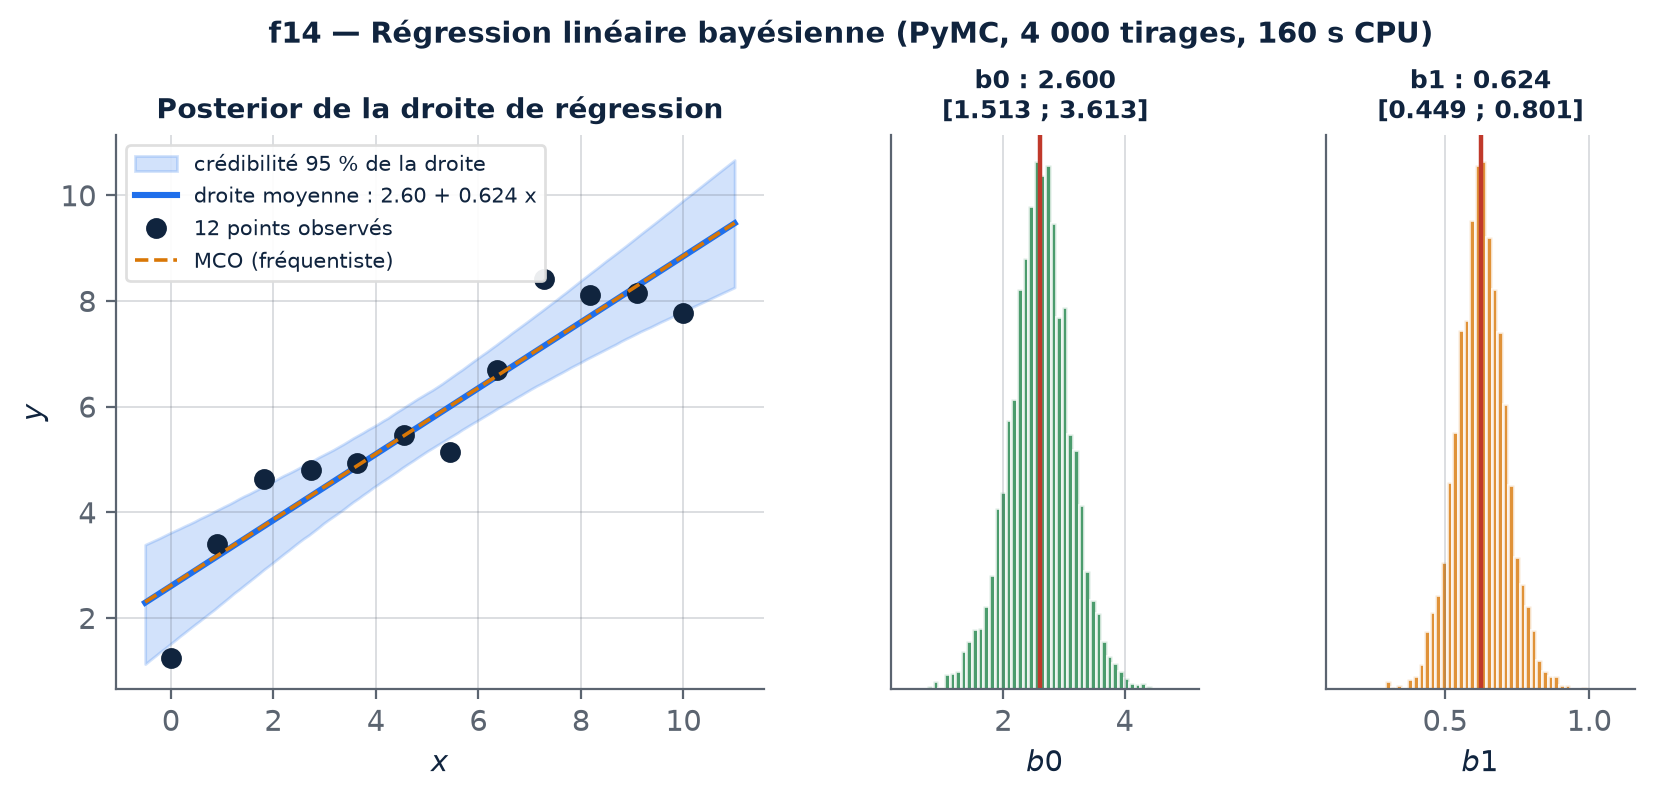
\includegraphics[width=.86\textwidth]{f14_regression_bayesienne.png}
\end{center}
\end{frame}

% [split]
\begin{frame}{Résultats réels (exécutés sur cette machine, CPU)}

\vspace{-1mm}
\begin{columns}[t]
\begin{column}{0.60\textwidth}
\begin{tabular}{@{}lccc@{}}
\toprule
Paramètre & Moyenne a post. & Crédibilité 95 \% & MCO (fréquentiste) \\
\midrule
$\beta_0$ (ordonnée) & 2,600 & $[1{,}513 \,;\, 3{,}613]$ & 2,611 \\
$\beta_1$ (pente) & 0,624 & $[0{,}449 \,;\, 0{,}801]$ & 0,624 \\
$\sigma$ (bruit) & 0,936 & --- & 0,92 \\
\bottomrule
\end{tabular}
\vspace{1mm}

\small Modèle échantillonné par NUTS : 2 chaînes, 4 000 tirages retenus,
$\hat R_{\max} = 1{,}0006$, 160 s sur un CPU 8 c\oe urs \emph{sans GPU}.
\end{column}
\begin{column}{0.38\textwidth}
\begin{kbox}[Apport du bayésien]
\begin{itemize}
  \item une \textbf{distribution} pour la pente, pas seulement un point ;
  \item $P(\beta_1 > 0 \given y) \approx 1$ : l'effet est certain ;
  \item avec 4 points au lieu de 12, MCO donnerait un IC énorme.

\end{itemize}
\end{kbox}
\end{column}
\end{columns}
\end{frame}

% ---------------------------------------------------------------- 34
% [split]
\begin{frame}{Prédire en bayésien : deux incertitudes, pas une}
\begin{center}
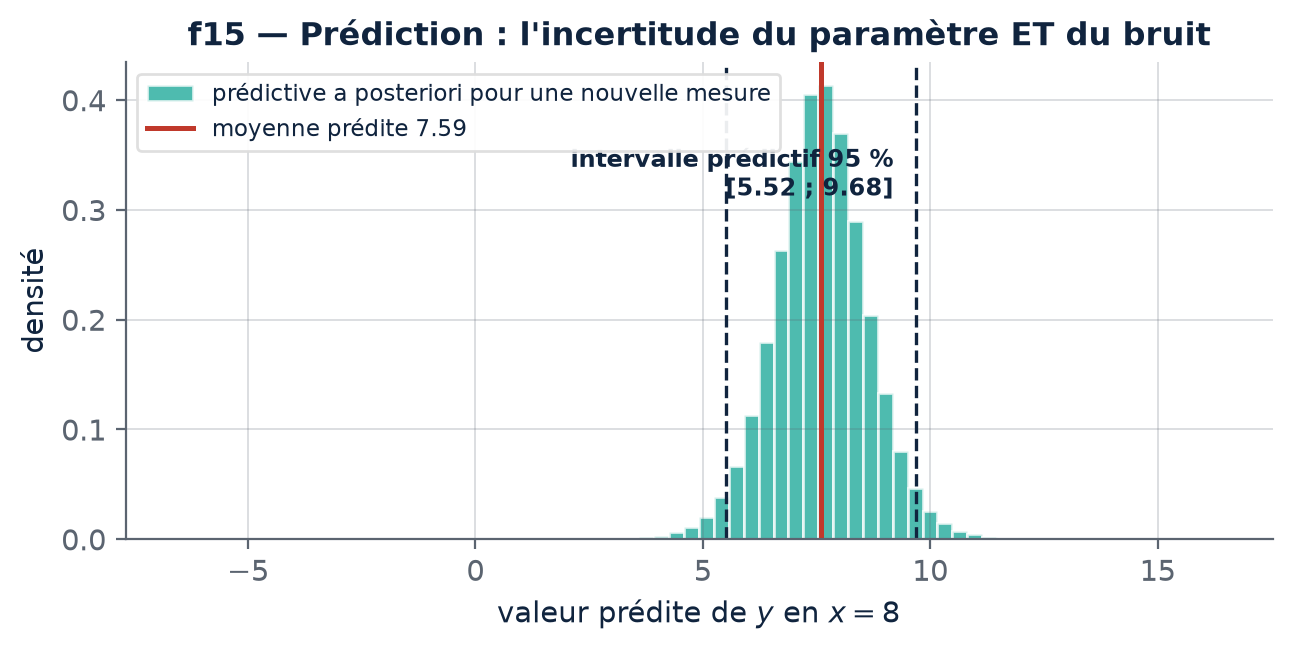
\includegraphics[width=\textwidth]{f15_prediction.png}
\end{center}
\end{frame}

% [split]
% [suite5]
\begin{frame}{Prédire en bayésien : deux incertitudes, pas une}
\begin{columns}[t]
\begin{column}{0.46\textwidth}
\begin{kbox}[La loi prédictive a posteriori]
\[
p(\tilde y \given y) = \int \underbrace{p(\tilde y \given \theta)}_{\text{bruit}}
\underbrace{p(\theta \given y)}_{\text{paramètre inconnu}} \mathrm{d}\theta
\]
On \textbf{intègre} sur l'incertitude du paramètre : la prédiction est
plus large qu'une prédiction faite à $\hat\theta$ fixé.
\end{kbox}
\begin{ebox}[Chiffres réels à $x = 8$]
\begin{itemize}
  \item valeur prédite moyenne : $7{,}59$
  \item crédibilité 95 \% de la \emph{moyenne} : $[6{,}83 \,;\, 8{,}40]$
  \item crédibilité 95 \% d'une \emph{observation} : $[5{,}52 \,;\, 9{,}68]$
\end{itemize}
\vspace{1mm}
\small L'écart entre les deux intervalles \textbf{est} la variabilité
$\sigma$ du processus : 0,94 ici.
\end{ebox}
\end{column}
\end{columns}
\end{frame}

% [suite5]
\begin{frame}{Prédire en bayésien : deux incertitudes, pas une (suite)}
\begin{wbox}[Erreur classique]
Confondre l'incertitude sur la \textbf{moyenne prédite} et celle sur la
\textbf{prochaine observation}. La seconde est toujours plus large et
c'est celle qui intéresse l'ingénieur.
\end{wbox}
\end{frame}

% ---------------------------------------------------------------- 35
\begin{frame}{Activité 2 — à vous de jouer (15 min)}
\begin{abox}[Consigne]
Par binôme, sur le jeu de données fourni \file{data/rendement\_12points.csv} (12 points,
colonnes \texttt{x} et \texttt{y}) :
\begin{enumerate}
  \item Refaites la régression de la slide précédente, mais avec un prior
        \textbf{très informatif} : $\beta_1 \sim \N(0{,}5, 0{,}05^2)$.
  \item Comparez la pente obtenue à celle du prior faiblement informatif.
  \item Que se passe-t-il si vous n'avez que les \textbf{4 premiers} points ?
        Le prior informatif aide-t-il ou trompe-t-il ?
  \item Rejouez l'analyse en doublant l'échelle de $x$ (convertissez $x$ en \% au lieu d'unités).
        Le prior sur $\beta_1$ devient-il raisonnable ?
\end{enumerate}
\end{abox}
\vspace{1mm}
\begin{columns}[t]
\begin{column}{0.48\textwidth}
\begin{kbox}[Ce que l'activité doit établir]
Un prior est \textbf{une hypothèse d'échelle}. Mal normalisé, il devient
une erreur silencieuse : le posterior sera précis et faux.
\end{kbox}
\end{column}
\begin{column}{0.48\textwidth}
\begin{kbox}[Indice]
Normaliser $x$ (centrer-réduire) rend les priors comparables entre études.
C'est la première recommandation pratique de Gelman.
\end{kbox}
\end{column}
\end{columns}
\end{frame}

% ---------------------------------------------------------------- 36
% [suite]
\begin{frame}{Correction collective et grille d'évaluation}
\begin{columns}[t]
\begin{column}{0.52\textwidth}
\begin{solbox}[Réponses attendues]
\begin{itemize}
  \item Prior $\N(0{,}5; 0{,}05^2)$ : le posterior de $\beta_1$ est
        \textbf{écrasé} autour de 0,5 (l'écart-type du prior est 10 fois trop petit).
  \item Avec 4 points seulement : le résultat suit le prior, l'intervalle de
        crédibilité est \emph{faussement étroit}. C'est le pire cas :
        \textbf{précis et faux}.
  \item En doublant l'échelle de $x$, la pente est divisée par 2 :
        le prior sur $\beta_1$ n'est plus adapté, il faut le renormaliser.
\end{itemize}
\end{solbox}
\end{column}
\begin{column}{0.46\textwidth}
{\setlength{\tabcolsep}{3pt}\begin{tabular}{@{}p{3.3cm}p{0.8cm}p{1.3cm}@{}}
\toprule
Critère d'évaluation & Points & Acquis ? \\
\midrule
Modèle PyMC correct et exécuté & 3 & \hspace{1.2cm} \\
Priors justifiés par écrit & 3 & \\
Comparaison chiffrée des deux priors & 3 & \\
Diagnostic de convergence ($\hat R$) & 2 & \\
Interprétation en une phrase & 3 & \\
Discussion de la sensibilité à l'échelle & 2 & \\
\midrule
\textbf{Total} & \textbf{16} & \\
\bottomrule
\end{tabular}}
\end{column}
\end{columns}
\vspace{1.5mm}
\end{frame}

% [suite]
\begin{frame}{Correction collective et grille d'évaluation (suite)}
\begin{wbox}[Le réflexe à acquérir]
Toujours se demander : \textbf{« mes données peuvent-elles seulement me contredire ? »}
Si non, votre prior est un dogme, pas un a priori.
\end{wbox}
\end{frame}

% ---------------------------------------------------------------- 37
\begin{frame}{Les deux écoles face au même jeu de données}
\begin{center}
\small
\begin{tabular}{@{}p{3.0cm}p{5.1cm}p{5.1cm}@{}}
\toprule
\textbf{Aspect} & \textbf{Fréquentiste} & \textbf{Bayésien} \\
\midrule
Ce qui est aléatoire & $\hat\theta$ (l'estimateur) sur des échantillons répétés
                     & $\theta$ (le paramètre) \\
Ce qui est fixe & $\theta$ & les données observées $y$ \\
Réponse donnée & point $+$ intervalle de confiance & distribution a posteriori \\
Question à laquelle on peut répondre & « si l'expérience était répétée \dots » &
« quelle est la plausibilité de ce que j'avance ? » \\
Information externe & non incorporable sans changer la méthode &
explicitée dans le prior \\
Arrêt anticipé & gonfle le risque de type I (sauf correction séquentielle) &
licite : la conclusion est conditionnelle aux données \\
Petits échantillons & inférence fragile, IC trompeur & le prior régularise
(\emph{shrinkage}) \\
Coût de calcul & faible (formules closes) & élevé (intégrales, MCMC) \\
Besoin de supervision & modèle seul & modèle \textbf{et} priors \\
\bottomrule
\end{tabular}
\end{center}
\vspace{1mm}
\begin{kbox}[La bonne posture]
Ce ne sont pas deux religions : ce sont deux façons de répondre à deux
\textbf{questions différentes}. Choisissez la question ; l'outil suivra.
\end{kbox}
\end{frame}

% ---------------------------------------------------------------- 38
% [rogna]
% [rogna]
% [rogna]
% [split]
\begin{frame}{La p-value n'est pas $P(H_0 \given \mathrm{données})$}
\begin{center}
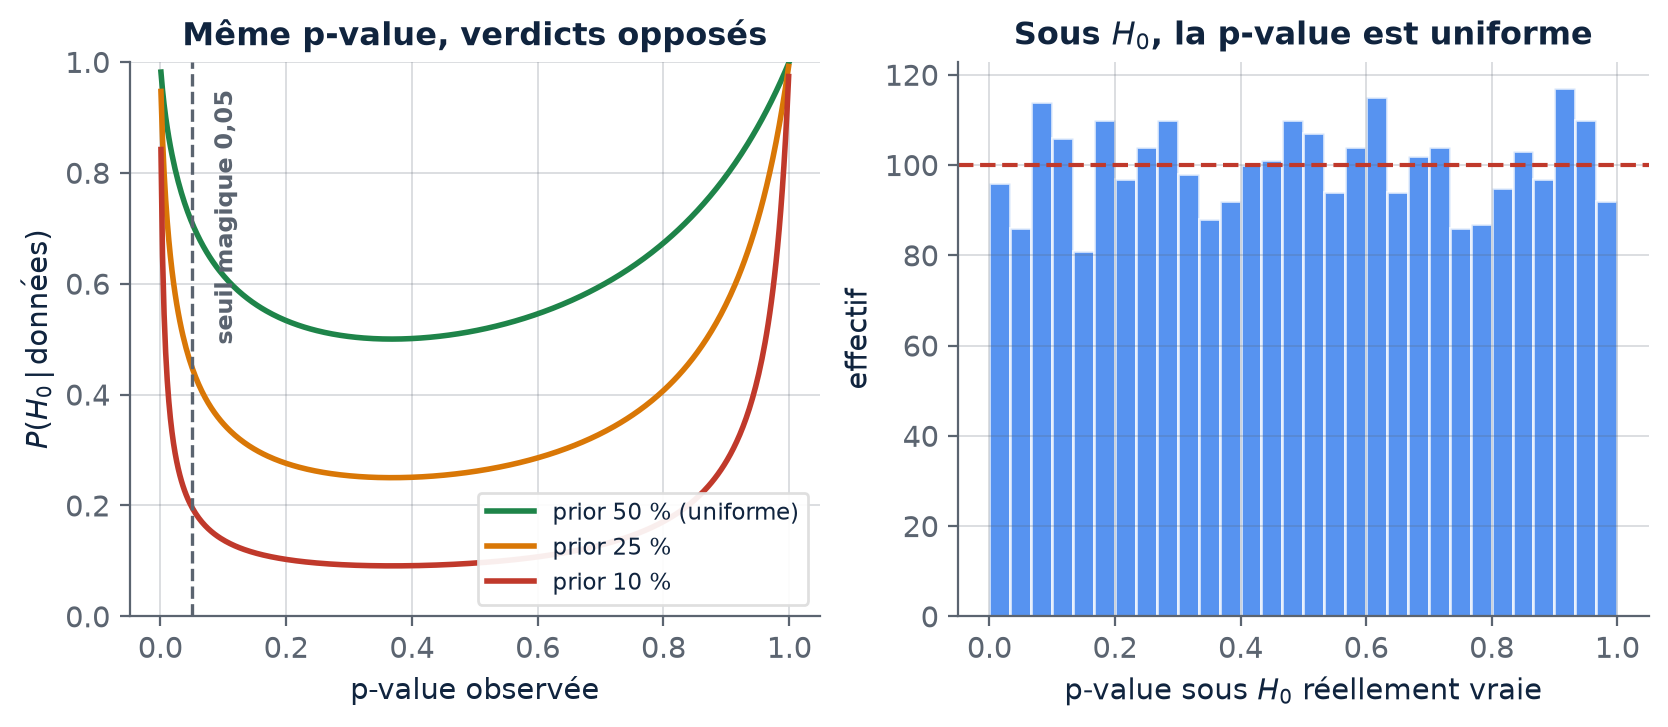
\includegraphics[width=.86\textwidth]{f08_pvalue_vs_posterior.png}
\end{center}
\end{frame}

% [split]
\begin{frame}{La p-value n'est pas $P(H_0 \given \mathrm{données})$}

\vspace{-1mm}
\begin{columns}[t]
\begin{column}{0.55\textwidth}
\begin{ebox}[Ce que la figure montre (calcul réel)]
Pour un test bilatéral, une p-value de $0{,}05$ \textbf{ne} signifie pas
« 5 \% de chance que $H_0$ soit vraie ». Avec un prior neutre
$P(H_0) = P(H_1) = 0{,}5$ et la calibration de Sellke--Johnson :
\[
BF_{01} \approx \frac{-1}{e\, p \log p} = 2{,}46
\;\Rightarrow\;
P(H_0 \given y) = 0{,}71
\]
\vspace{1mm}
\small Avec 10 \% de prior sur $H_0$ : $P(H_0 \given y) = 0{,}21$ ; avec 90 \% : $0{,}96$.
\textbf{Même p-value, trois conclusions.}
\end{ebox}
\end{column}
\begin{column}{0.43\textwidth}
\begin{kbox}[La formule à retenir]
$P(H_0 \given y)$ dépend de deux choses et de deux seulement :
\begin{itemize}
  \item ce que l'on croyait \textbf{avant} ($P(H_0)$) ;
  \item la force de l'évidence ($BF_{01}$).
\end{itemize}
La p-value ne contient que la seconde.
\end{kbox}
\end{column}
\end{columns}
\end{frame}

% ---------------------------------------------------------------- 27
\begin{frame}[fragile]{Boîte à outils : la fonction qui fait tout}
% [rogna]
\small
\begin{columns}[t]
\begin{column}{0.53\textwidth}
\begin{codebox}[bayes.py — version minimale et générale]
\begin{lstlisting}
import numpy as np
from scipy import stats

def posterior_discret(prior_grid, prior_pdf, vraisemblance, y):
    """Posterior sur une grille : suffit des que theta est
    de dimension 1 ou 2. Aucune formule close requise."""
    post = prior_pdf(prior_grid) * vraisemblance(prior_grid, y)
    post /= np.trapezoid(post, prior_grid)     # normalisation
    return post

def proba(prior_grid, post, seuil):
    """P(theta > seuil | y) : LA question a laquelle le
    frequentiste ne peut pas repondre."""
    m = prior_grid > seuil
    return np.trapezoid(post[m], prior_grid[m])

def intervale_credibilite(prior_grid, post, niveau=0.95):
    c = np.cumsum(post) / post.sum()
    lo = prior_grid[np.searchsorted(c, (1 - niveau) / 2)]
    hi = prior_grid[np.searchsorted(c, 1 - (1 - niveau) / 2)]
    return lo, hi
\end{lstlisting}
\end{codebox}
\end{column}
\begin{column}{0.45\textwidth}
\begin{kbox}[Trois fonctions, tout le chapitre]
\begin{itemize}
  \item \textbf{grille $+$ normalisation} : la méthode universelle quand
        aucune conjugaison n'est disponible ;
  \item \textbf{proba dépassant un seuil} : la question décisionnelle ;
  \item \textbf{intervalle de crédibilité} : la synthèse de l'incertitude.
\end{itemize}
\end{kbox}
\begin{wbox}[Quand la grille ne suffit plus]
En dimension $d$, une grille coûte $n^d$ points : impossible au-delà de
$d \approx 3$. C'est \textbf{exactement} le mur qui a motivé les méthodes MCMC
(chapitre 5).
\end{wbox}
\end{column}
\end{columns}
\end{frame}

% ---------------------------------------------------------------- 28
\begin{frame}{Ce qui change quand le paramètre devient continu}
\begin{columns}[t]
\begin{column}{0.49\textwidth}
\begin{ebox}[Cas continu, exemple complet]
Mesures répétées d'une grandeur physique, $y_i \sim \N(\mu, \sigma^2)$ avec
$\sigma$ connu :
\[
\begin{aligned}
p(\mu) &= \N(\mu_0, \tau_0^2) \quad\text{(prior)}\\
p(y \given \mu) &\propto \prod_{i=1}^n e^{-\frac{(y_i-\mu)^2}{2\sigma^2}}\\
&\propto e^{-\frac{n(\bar y - \mu)^2}{2\sigma^2}}
\end{aligned}
\]
Le posterior est encore \textbf{normal} : $\N(\mu_n, \tau_n^2)$ avec
\[
\frac{1}{\tau_n^2} = \frac{1}{\tau_0^2} + \frac{n}{\sigma^2}
\]
\end{ebox}
\end{column}
\begin{column}{0.49\textwidth}
\begin{kbox}[Lecture : la précision s'additionne]
Ce n'est pas $\mu$ qui s'additionne, c'est l'\textbf{information}
$1/$variance. Le posterior est la moyenne pondérée des deux sources,
avec les poids $1/\tau_0^2$ et $n/\sigma^2$.
\vspace{1mm}
\[
\mu_n = \frac{\frac{\mu_0}{\tau_0^2}+\frac{n\bar y}{\sigma^2}}{\frac{1}{\tau_0^2}+\frac{n}{\sigma^2}}
\]
\end{kbox}
\begin{ebox}[Chiffres]
Avec $\mu_0 = 100$, $\tau_0 = 10$, $\sigma = 5$, $n = 4$, $\bar y = 92$ :
$\mu_n = 93{,}3$ et $\tau_n = 2{,}44$.
Le prior pèse encore, mais les données dominent déjà.
\end{ebox}
\end{column}
\end{columns}
\end{frame}

% ---------------------------------------------------------------- 29
% [suite]
\begin{frame}{La constante de normalisation : pourquoi on l'ignore}
\begin{columns}[t]
\begin{column}{0.52\textwidth}
\begin{kbox}[Le raisonnement]
\[
p(\theta \given y) = \frac{p(y \given \theta)p(\theta)}{\underbrace{p(y)}_{\text{indépendant de }\theta}}
\]
$p(y)$ est le \emph{même nombre} pour toutes les valeurs de $\theta$ :
il \textbf{recentre} la courbe, il ne la \textbf{redessine} pas. Pour
comparer deux valeurs de $\theta$, il disparaît.
\end{kbox}
\begin{ebox}[Ordre de grandeur]
Dans l'exemple Beta-Binomial, $p(y)$ vaut exactement
$P(Y = 7)$ sous la loi prédictive a priori :
\[
p(y) = \binom{10}{7}\frac{\Gamma(2)\Gamma(11)}{\Gamma(13)} = \frac{1}{12} = 0{,}0833
\]
Le posterior $\mathrm{Beta}(8,4)$ divisé par ce facteur redonne bien une densité d'aire 1.
\end{ebox}
\end{column}
\begin{column}{0.46\textwidth}
\begin{wbox}[Ne l'oubliez jamais : il revient]
$p(y)$ réapparaît dans trois situations \textbf{décisives} :
\begin{itemize}
  \item \textbf{Comparer deux modèles} : c'est le facteur de Bayes
        $BF_{12} = p(y \given M_1)/p(y \given M_2)$ (chapitre 4) ;
  \item \textbf{Choisir un prior} : $p(y)$ mesure la \emph{plausibilité}
        du prior avant de voir les données (checks prédictifs a priori) ;
  \item \textbf{Modèles hiérarchiques} : il faut intégrer les effets
        latents pour évaluer la vraisemblance marginale.
\end{itemize}
\end{wbox}
\end{column}
\end{columns}
\end{frame}

% [suite]
\begin{frame}{La constante de normalisation : pourquoi on l'ignore (suite)}
\begin{kbox}[Règle pratique]
On travaille en \textbf{logarithme} :
$\log p(\theta \given y) = \log p(y \given \theta) + \log p(\theta) + \text{cte}$.
Toute l'inférence numérique (grilles, MCMC, VI) optimise ou échantillonne ce log-posterior.
\end{kbox}

\end{frame}

% ---------------------------------------------------------------- 30
\begin{frame}{Le mécanisme : une multiplication, pas une recette}
\begin{center}
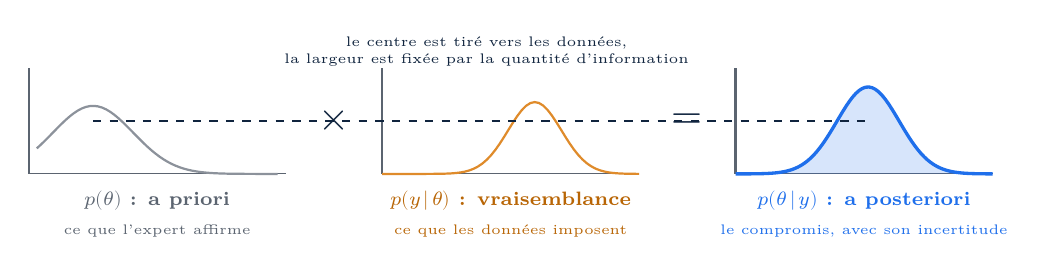
\begin{tikzpicture}[xscale=1.02,yscale=.96]
% --- prior
\draw[byGrey,thin] (-0.1,0) -- (3.1,0);
\draw[-,thick,byGrey] (-0.1,0) -- (-0.1,1.4);
\draw[byGrey!70,thick,domain=0:3,samples=60] plot (\x,{0.9*exp(-((\x-0.7)^2)/0.5)});
\node[byGrey,font=\scriptsize\bfseries] at (1.5,-0.35) {$p(\theta)$ : a priori};
\node[byGrey,font=\tiny] at (1.5,-0.75) {ce que l'expert affirme};
% --- x
\node[byDeep,font=\Large\bfseries] at (3.7,0.7) {$\times$};
% --- vraisemblance
\draw[byGrey,thin] (4.3,0) -- (7.5,0);
\draw[-,thick,byGrey] (4.3,0) -- (4.3,1.4);
\draw[byOrange!85,thick,domain=4.3:7.5,samples=60]
   plot (\x,{0.95*exp(-((\x-6.2)^2)/0.22)});
\node[byOrange!85!black,font=\scriptsize\bfseries] at (5.9,-0.35) {$p(y \given \theta)$ : vraisemblance};
\node[byOrange!85!black,font=\tiny] at (5.9,-0.75) {ce que les données imposent};
% --- =
\node[byDeep,font=\Large\bfseries] at (8.1,0.7) {$=$};
% --- posterior
\draw[byGrey,thin] (8.7,0) -- (11.9,0);
\draw[-,thick,byGrey] (8.7,0) -- (8.7,1.4);
\draw[byBlue,very thick,domain=8.7:11.9,samples=80]
   plot (\x,{1.15*exp(-((\x-10.35)^2)/0.30)});
\fill[byBlue,opacity=.18,domain=8.7:11.9,samples=80]
   (8.7,0) -- plot (\x,{1.15*exp(-((\x-10.35)^2)/0.30)}) -- (11.9,0) -- cycle;
\node[byBlue,font=\scriptsize\bfseries] at (10.3,-0.35) {$p(\theta \given y)$ : a posteriori};
\node[byBlue,font=\tiny] at (10.3,-0.75) {le compromis, avec son incertitude};
% --- annotations
\draw[byDeep,dashed,thin] (0.7,0.7) -- (10.35,0.7);
\node[byDeep,font=\tiny,align=center] at (5.6,1.62) {le centre est tiré vers les données, \\ la largeur est fixée par la quantité d'information};
\end{tikzpicture}
\end{center}
\vspace{1mm}
\begin{columns}[t]
\begin{column}{0.48\textwidth}
\begin{kbox}[Trois cas]
\begin{itemize}
  \item $\,$ prior étroit, données rares $\Rightarrow$ le prior gagne ;
  \item prior large, données nombreuses $\Rightarrow$ les données gagnent ;
  \item les deux étroits et \textbf{déplacés} $\Rightarrow$ conflit prior/données :
        \textbf{signalez-le}, ne le cachez pas.
\end{itemize}
\end{kbox}
\end{column}
\begin{column}{0.48\textwidth}
\begin{abox}[Démonstration en direct]
On rejoue la même figure avec $\alpha,\beta$ modifiables et
$n$ croissant dans le notebook
\file{TP1\_mise\_a\_jour\_\allowbreak bayesienne.ipynb} (dossier \file{notebooks/}), section 4.
\end{abox}
\end{column}
\end{columns}
\end{frame}

% ---------------------------------------------------------------- 31
\begin{frame}{Mise à jour séquentielle : la version formelle}
\begin{columns}[t]
\begin{column}{0.5\textwidth}
\begin{kbox}[Traitement par lot]
\[
p(\theta \given y_1,\dots,y_n) \propto p(\theta)\prod_{i=1}^{n}p(y_i \given \theta)
\]
\end{kbox}
\begin{kbox}[Traitement en flux (= c'est pareil)]
\[
\begin{aligned}
p(\theta \given y_1) &\propto p(\theta)\,p(y_1 \given \theta)\\
p(\theta \given y_1,y_2) &\propto p(\theta \given y_1)\,p(y_2 \given \theta)\\
&\;\;\vdots
\end{aligned}
\]
Aucune information n'est perdue : le posterior contient
\emph{toute} l'information apportée par les données déjà vues.
\end{kbox}
\end{column}
\begin{column}{0.48\textwidth}
\begin{ebox}[Conséquence majeure]
Un modèle bayésien peut être \textbf{actualisé en continu} : c'est ce qui
rend le filtrage de Kalman, les bandits bayésiens, l'arrêt anticipé des essais
cliniques et l'A/B testing séquentiel possibles \emph{sans pénalité de multiplicité}.
\end{ebox}
\begin{wbox}[Attention au raccourci]
« Le posterior suffit » n'est vrai que si le \textbf{modèle} est resté le même.
Changer de modèle (ajouter une covariable, abandonner la normalité) impose de
réévaluer le prior et la vraisemblance : le posterior d'un modèle A n'est
pas le prior d'un modèle B.
\end{wbox}
\end{column}
\end{columns}
\end{frame}

% ---------------------------------------------------------------- 32
\begin{frame}[fragile]{Exemple complet : régression linéaire bayésienne}
\begin{columns}[t]
\begin{column}{0.5\textwidth}
\begin{ebox}[Données et modèle]
12 mesures d'un rendement $y$ en fonction d'une dose $x$ (0 à 10).
\[
y_i = \beta_0 + \beta_1 x_i + \varepsilon_i, \qquad
\varepsilon_i \sim \N(0, \sigma^2)
\]
Priors \textbf{faiblement informatifs} :
\[
\beta_0 \sim \N(0, 5^2),\quad
\beta_1 \sim \N(0{,}5, 1^2),\quad
\sigma \sim \text{Demi-Normale}(2)
\]
\end{ebox}
\begin{kbox}[Pourquoi ces priors ?]
Volontairement larges : ils n'imposent rien de précis, mais ils
\textbf{empêchent des valeurs absurdes} (une pente de $10^6$). Ils disent
« je m'attends à un effet modéré, dans un ordre de grandeur raisonnable ».
\end{kbox}
\end{column}
\begin{column}{0.48\textwidth}
\begin{codebox}[PyMC — le modèle complet]
\begin{lstlisting}
with pm.Model() as modele:
    b0 = pm.Normal("b0", mu=0, sigma=5)
    b1 = pm.Normal("b1", mu=0.5, sigma=1)
    sigma = pm.HalfNormal("sigma", sigma=2)
    mu = b0 + b1 * x
    pm.Normal("y", mu=mu, sigma=sigma, observed=y)
    trace = pm.sample(draws=2000, tune=1500, chains=2)
\end{lstlisting}
\end{codebox}
\begin{abox}[Ce que l'on va lire sur le résultat]
\begin{itemize}
  \item la postérieure de chaque coefficient ;
  \item l'intervalle de crédibilité à 95 \% ;
  \item la prévision \textbf{avec} son incertitude.
\end{itemize}
\end{abox}
\end{column}
\end{columns}
\end{frame}

% ---------------------------------------------------------------- 33
% [rogna]
% [split]
\begin{frame}{Résultats réels (exécutés sur cette machine, CPU)}
\begin{center}
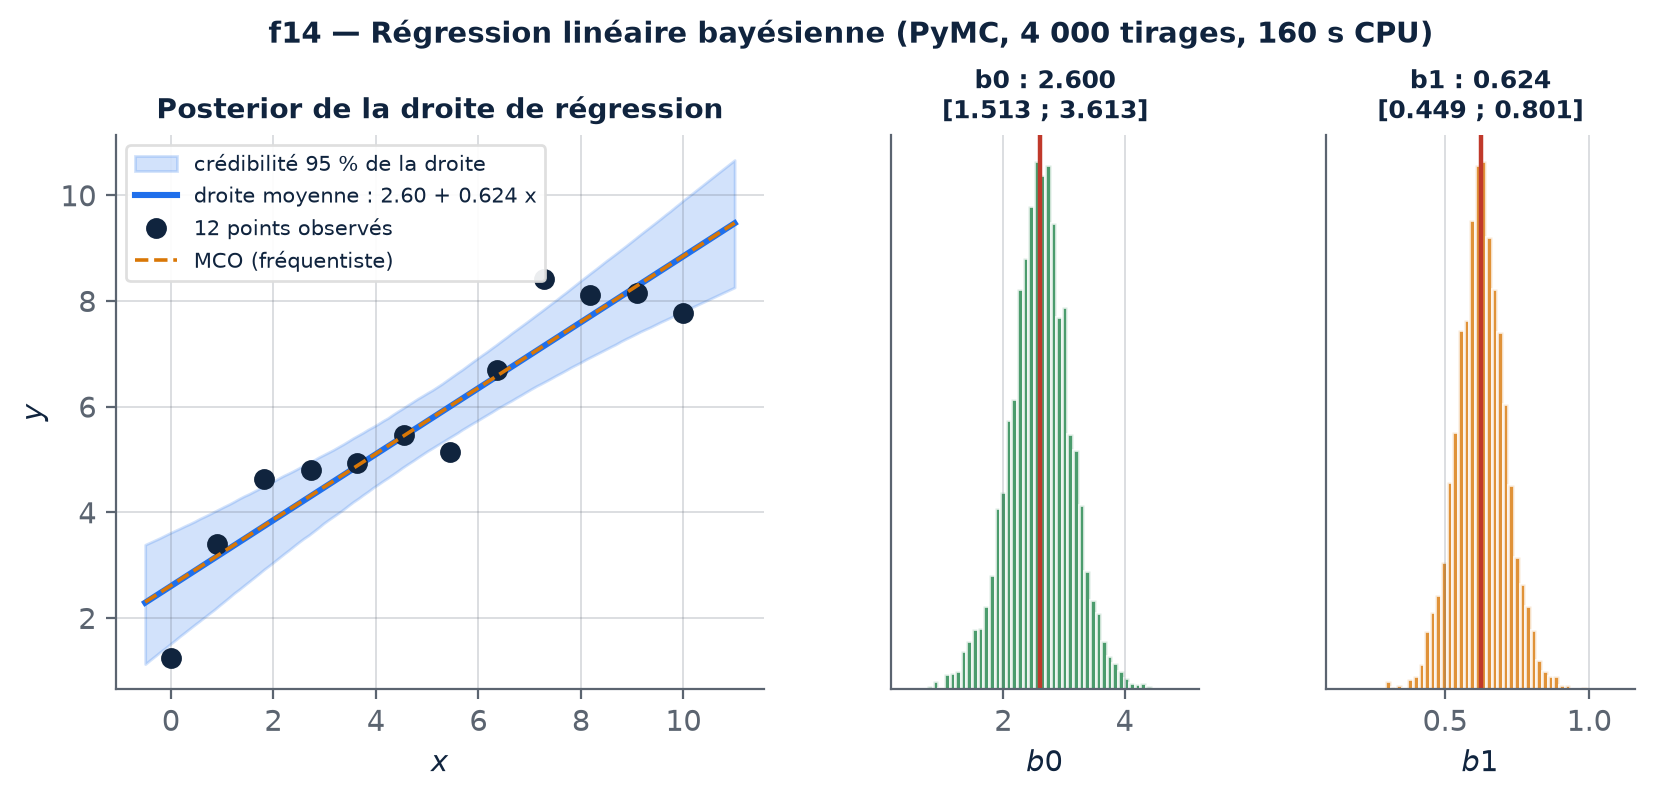
\includegraphics[width=.86\textwidth]{f14_regression_bayesienne.png}
\end{center}
\end{frame}

% [split]
\begin{frame}{Résultats réels (exécutés sur cette machine, CPU)}

\vspace{-1mm}
\begin{columns}[t]
\begin{column}{0.60\textwidth}
\begin{tabular}{@{}lccc@{}}
\toprule
Paramètre & Moyenne a post. & Crédibilité 95 \% & MCO (fréquentiste) \\
\midrule
$\beta_0$ (ordonnée) & 2,600 & $[1{,}513 \,;\, 3{,}613]$ & 2,611 \\
$\beta_1$ (pente) & 0,624 & $[0{,}449 \,;\, 0{,}801]$ & 0,624 \\
$\sigma$ (bruit) & 0,936 & --- & 0,92 \\
\bottomrule
\end{tabular}
\vspace{1mm}

\small Modèle échantillonné par NUTS : 2 chaînes, 4 000 tirages retenus,
$\hat R_{\max} = 1{,}0006$, 160 s sur un CPU 8 c\oe urs \emph{sans GPU}.
\end{column}
\begin{column}{0.38\textwidth}
\begin{kbox}[Apport du bayésien]
\begin{itemize}
  \item une \textbf{distribution} pour la pente, pas seulement un point ;
  \item $P(\beta_1 > 0 \given y) \approx 1$ : l'effet est certain ;
  \item avec 4 points au lieu de 12, MCO donnerait un IC énorme.

\end{itemize}
\end{kbox}
\end{column}
\end{columns}
\end{frame}

% ---------------------------------------------------------------- 34
% [split]
\begin{frame}{Prédire en bayésien : deux incertitudes, pas une}
\begin{center}
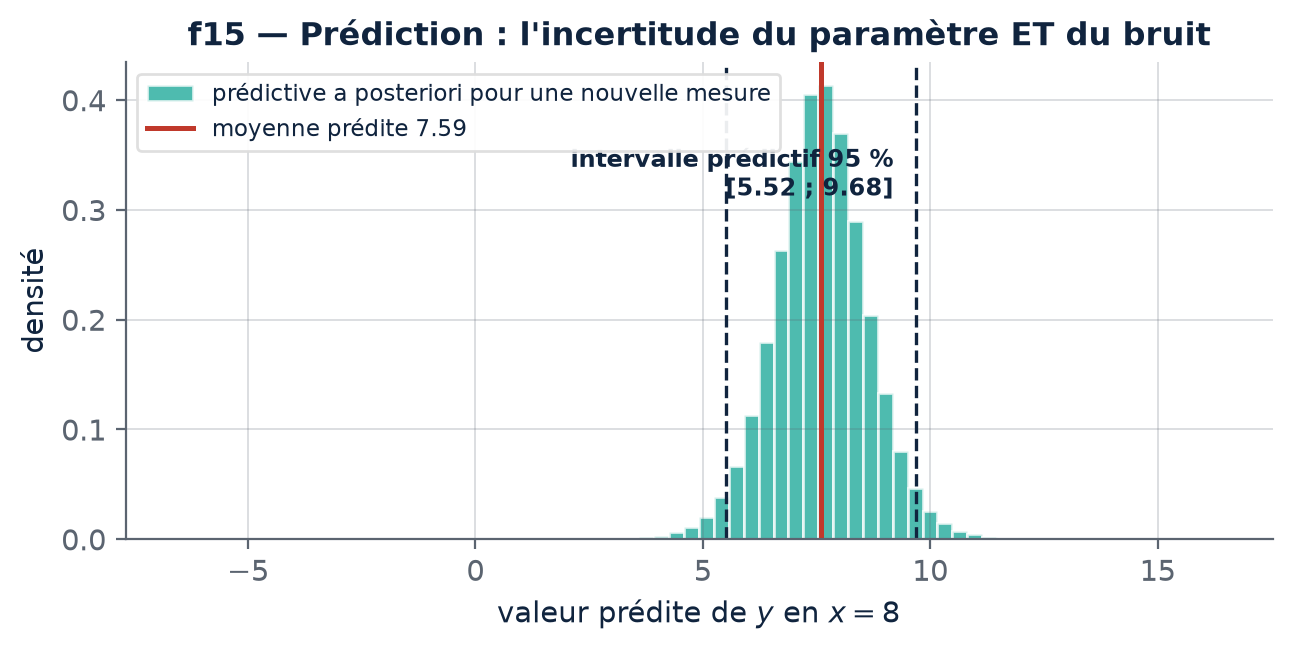
\includegraphics[width=\textwidth]{f15_prediction.png}
\end{center}
\end{frame}

% [split]
\begin{frame}{Prédire en bayésien : deux incertitudes, pas une}
\begin{columns}[t]
\begin{column}{0.46\textwidth}
\begin{kbox}[La loi prédictive a posteriori]
\[
p(\tilde y \given y) = \int \underbrace{p(\tilde y \given \theta)}_{\text{bruit}}
\underbrace{p(\theta \given y)}_{\text{paramètre inconnu}} \mathrm{d}\theta
\]
On \textbf{intègre} sur l'incertitude du paramètre : la prédiction est
plus large qu'une prédiction faite à $\hat\theta$ fixé.
\end{kbox}
\begin{ebox}[Chiffres réels à $x = 8$]
\begin{itemize}
  \item valeur prédite moyenne : $7{,}59$
  \item crédibilité 95 \% de la \emph{moyenne} : $[6{,}83 \,;\, 8{,}40]$
  \item crédibilité 95 \% d'une \emph{observation} : $[5{,}52 \,;\, 9{,}68]$
\end{itemize}
\vspace{1mm}
\small L'écart entre les deux intervalles \textbf{est} la variabilité
$\sigma$ du processus : 0,94 ici.
\end{ebox}
\begin{wbox}[Erreur classique]
Confondre l'incertitude sur la \textbf{moyenne prédite} et celle sur la
\textbf{prochaine observation}. La seconde est toujours plus large et
c'est celle qui intéresse l'ingénieur.
\end{wbox}
\end{column}
\end{columns}
\end{frame}

% ---------------------------------------------------------------- 35
\begin{frame}{Activité 2 — à vous de jouer (15 min)}
\begin{abox}[Consigne]
Par binôme, sur le jeu de données fourni \file{data/rendement\_12points.csv} (12 points,
colonnes \texttt{x} et \texttt{y}) :
\begin{enumerate}
  \item Refaites la régression de la slide précédente, mais avec un prior
        \textbf{très informatif} : $\beta_1 \sim \N(0{,}5, 0{,}05^2)$.
  \item Comparez la pente obtenue à celle du prior faiblement informatif.
  \item Que se passe-t-il si vous n'avez que les \textbf{4 premiers} points ?
        Le prior informatif aide-t-il ou trompe-t-il ?
  \item Rejouez l'analyse en doublant l'échelle de $x$ (convertissez $x$ en \% au lieu d'unités).
        Le prior sur $\beta_1$ devient-il raisonnable ?
\end{enumerate}
\end{abox}
\vspace{1mm}
\begin{columns}[t]
\begin{column}{0.48\textwidth}
\begin{kbox}[Ce que l'activité doit établir]
Un prior est \textbf{une hypothèse d'échelle}. Mal normalisé, il devient
une erreur silencieuse : le posterior sera précis et faux.
\end{kbox}
\end{column}
\begin{column}{0.48\textwidth}
\begin{kbox}[Indice]
Normaliser $x$ (centrer-réduire) rend les priors comparables entre études.
C'est la première recommandation pratique de Gelman.
\end{kbox}
\end{column}
\end{columns}
\end{frame}

% ---------------------------------------------------------------- 36
% [suite]
\begin{frame}{Correction collective et grille d'évaluation}
\begin{columns}[t]
\begin{column}{0.52\textwidth}
\begin{solbox}[Réponses attendues]
\begin{itemize}
  \item Prior $\N(0{,}5; 0{,}05^2)$ : le posterior de $\beta_1$ est
        \textbf{écrasé} autour de 0,5 (l'écart-type du prior est 10 fois trop petit).
  \item Avec 4 points seulement : le résultat suit le prior, l'intervalle de
        crédibilité est \emph{faussement étroit}. C'est le pire cas :
        \textbf{précis et faux}.
  \item En doublant l'échelle de $x$, la pente est divisée par 2 :
        le prior sur $\beta_1$ n'est plus adapté, il faut le renormaliser.
\end{itemize}
\end{solbox}
\end{column}
\begin{column}{0.46\textwidth}
{\setlength{\tabcolsep}{3pt}\begin{tabular}{@{}p{3.3cm}p{0.8cm}p{1.3cm}@{}}
\toprule
Critère d'évaluation & Points & Acquis ? \\
\midrule
Modèle PyMC correct et exécuté & 3 & \hspace{1.2cm} \\
Priors justifiés par écrit & 3 & \\
Comparaison chiffrée des deux priors & 3 & \\
Diagnostic de convergence ($\hat R$) & 2 & \\
Interprétation en une phrase & 3 & \\
Discussion de la sensibilité à l'échelle & 2 & \\
\midrule
\textbf{Total} & \textbf{16} & \\
\bottomrule
\end{tabular}}
\end{column}
\end{columns}
\vspace{1.5mm}
\end{frame}

% [suite]
\begin{frame}{Correction collective et grille d'évaluation (suite)}
\begin{wbox}[Le réflexe à acquérir]
Toujours se demander : \textbf{« mes données peuvent-elles seulement me contredire ? »}
Si non, votre prior est un dogme, pas un a priori.
\end{wbox}
\end{frame}

% ---------------------------------------------------------------- 37
\begin{frame}{Les deux écoles face au même jeu de données}
\begin{center}
\small
\begin{tabular}{@{}p{3.0cm}p{5.1cm}p{5.1cm}@{}}
\toprule
\textbf{Aspect} & \textbf{Fréquentiste} & \textbf{Bayésien} \\
\midrule
Ce qui est aléatoire & $\hat\theta$ (l'estimateur) sur des échantillons répétés
                     & $\theta$ (le paramètre) \\
Ce qui est fixe & $\theta$ & les données observées $y$ \\
Réponse donnée & point $+$ intervalle de confiance & distribution a posteriori \\
Question à laquelle on peut répondre & « si l'expérience était répétée \dots » &
« quelle est la plausibilité de ce que j'avance ? » \\
Information externe & non incorporable sans changer la méthode &
explicitée dans le prior \\
Arrêt anticipé & gonfle le risque de type I (sauf correction séquentielle) &
licite : la conclusion est conditionnelle aux données \\
Petits échantillons & inférence fragile, IC trompeur & le prior régularise
(\emph{shrinkage}) \\
Coût de calcul & faible (formules closes) & élevé (intégrales, MCMC) \\
Besoin de supervision & modèle seul & modèle \textbf{et} priors \\
\bottomrule
\end{tabular}
\end{center}
\vspace{1mm}
\begin{kbox}[La bonne posture]
Ce ne sont pas deux religions : ce sont deux façons de répondre à deux
\textbf{questions différentes}. Choisissez la question ; l'outil suivra.
\end{kbox}
\end{frame}

% ---------------------------------------------------------------- 38
% [rogna]
% [rogna]
% [rogna]
% [split]
\begin{frame}{La p-value n'est pas $P(H_0 \given \mathrm{données})$}
\begin{center}
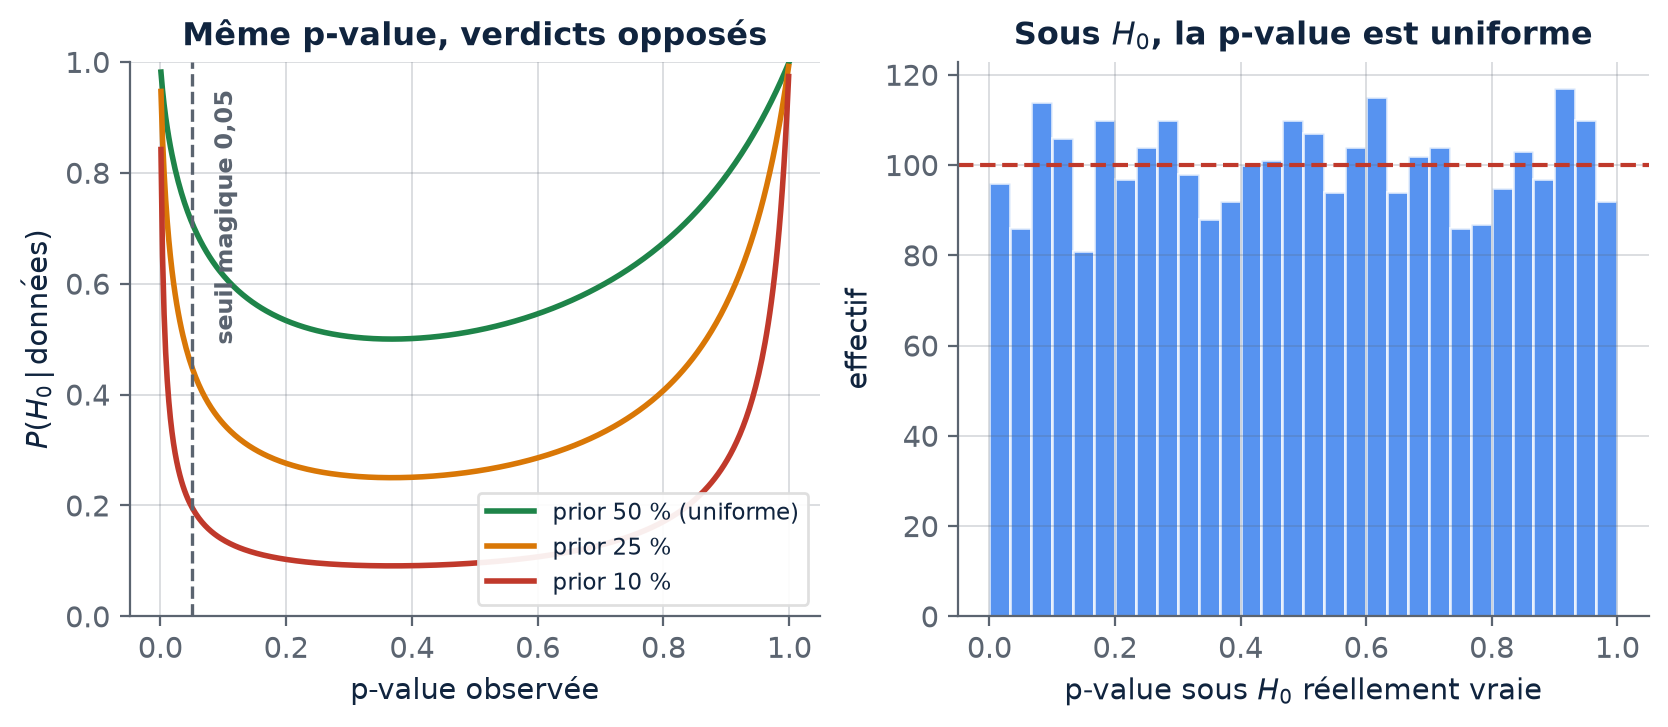
\includegraphics[width=.86\textwidth]{f08_pvalue_vs_posterior.png}
\end{center}
\end{frame}

% [split]
\begin{frame}{La p-value n'est pas $P(H_0 \given \mathrm{données})$}

\vspace{-1mm}
\begin{columns}[t]
\begin{column}{0.55\textwidth}
\begin{ebox}[Ce que la figure montre (calcul réel)]
Pour un test bilatéral, une p-value de $0{,}05$ \textbf{ne} signifie pas
« 5 \% de chance que $H_0$ soit vraie ». Avec un prior neutre
$P(H_0) = P(H_1) = 0{,}5$ et la calibration de Sellke--Johnson :
\[
BF_{01} \approx \frac{-1}{e\, p \log p} = 2{,}46
\;\Rightarrow\;
P(H_0 \given y) = 0{,}71
\]
\vspace{1mm}
\small Avec 10 \% de prior sur $H_0$ : $P(H_0 \given y) = 0{,}21$ ; avec 90 \% : $0{,}96$.
\textbf{Même p-value, trois conclusions.}
\end{ebox}
\end{column}
\begin{column}{0.43\textwidth}
\begin{kbox}[La formule à retenir]
$P(H_0 \given y)$ dépend de deux choses et de deux seulement :
\begin{itemize}
  \item ce que l'on croyait \textbf{avant} ($P(H_0)$) ;
  \item la force de l'évidence ($BF_{01}$).
\end{itemize}
La p-value ne contient que la seconde.
\end{kbox}
\end{column}
\end{columns}
\end{frame}
\end{document}
